\section{Hours of Operation and Occupancy}
\label{sec:hoo}

\subsection{Hours of Operation}
\subsubsection{Overview}
Hours of operation are added to the model using operation start time and duration inputs. The start times and durations are assigned to each model through the sampling process using a set of distributions based on building type. They are then further broken down by weekday and weekend (Figure~\ref{fig:start_time} and Figure~\ref{fig:duration}). When applied to the model, the start time and duration are used to establish operating hour start and end times. These times are used to adjust the other schedules in the model (e.g., lighting, thermostat). This is achieved by stretching or shrinking the schedule on the temporal axis to align all schedules with the operating hours for the model. Note that because the weekday and weekend start times and durations are sampled independently, they are not aligned in a given building model.

\subsubsection{Hours of Operation Derivation}
We derived the hours of operation by applying the method introduced in \cite{bianchi2020modeling} to 1 year of AMI data from 6,070 buildings spread across eight utilities (the commercial schedules AMI data set). We first extracted the two-dimensional distribution of \textit{High Load Start Time} and \textit{High Load Duration} from this AMI data set, as an approximation of the schedule of hours of operations for each building type. Then, we compared this distribution with the inputs of ComStock at the start of 
 the \href{https://www.nrel.gov/buildings/end-use-load-profiles.html}{End-Use Load Profiles} (EULP) calibration.

Figure~\ref{fig:utility_building_type} lists the number of buildings for each building type from each utility's AMI data set that was considered during the EULP project. The utility data sets and names are listed in Table 10 of the EULP Final Technical Report \citep{eulp_final_report}. Among the 15 building types considered in ComStock, 14 can be found in the commercial schedules AMI data set. The only exception is secondary schools, because all schools were grouped together in the AMI data.

%\begin{figure}
%    \centering 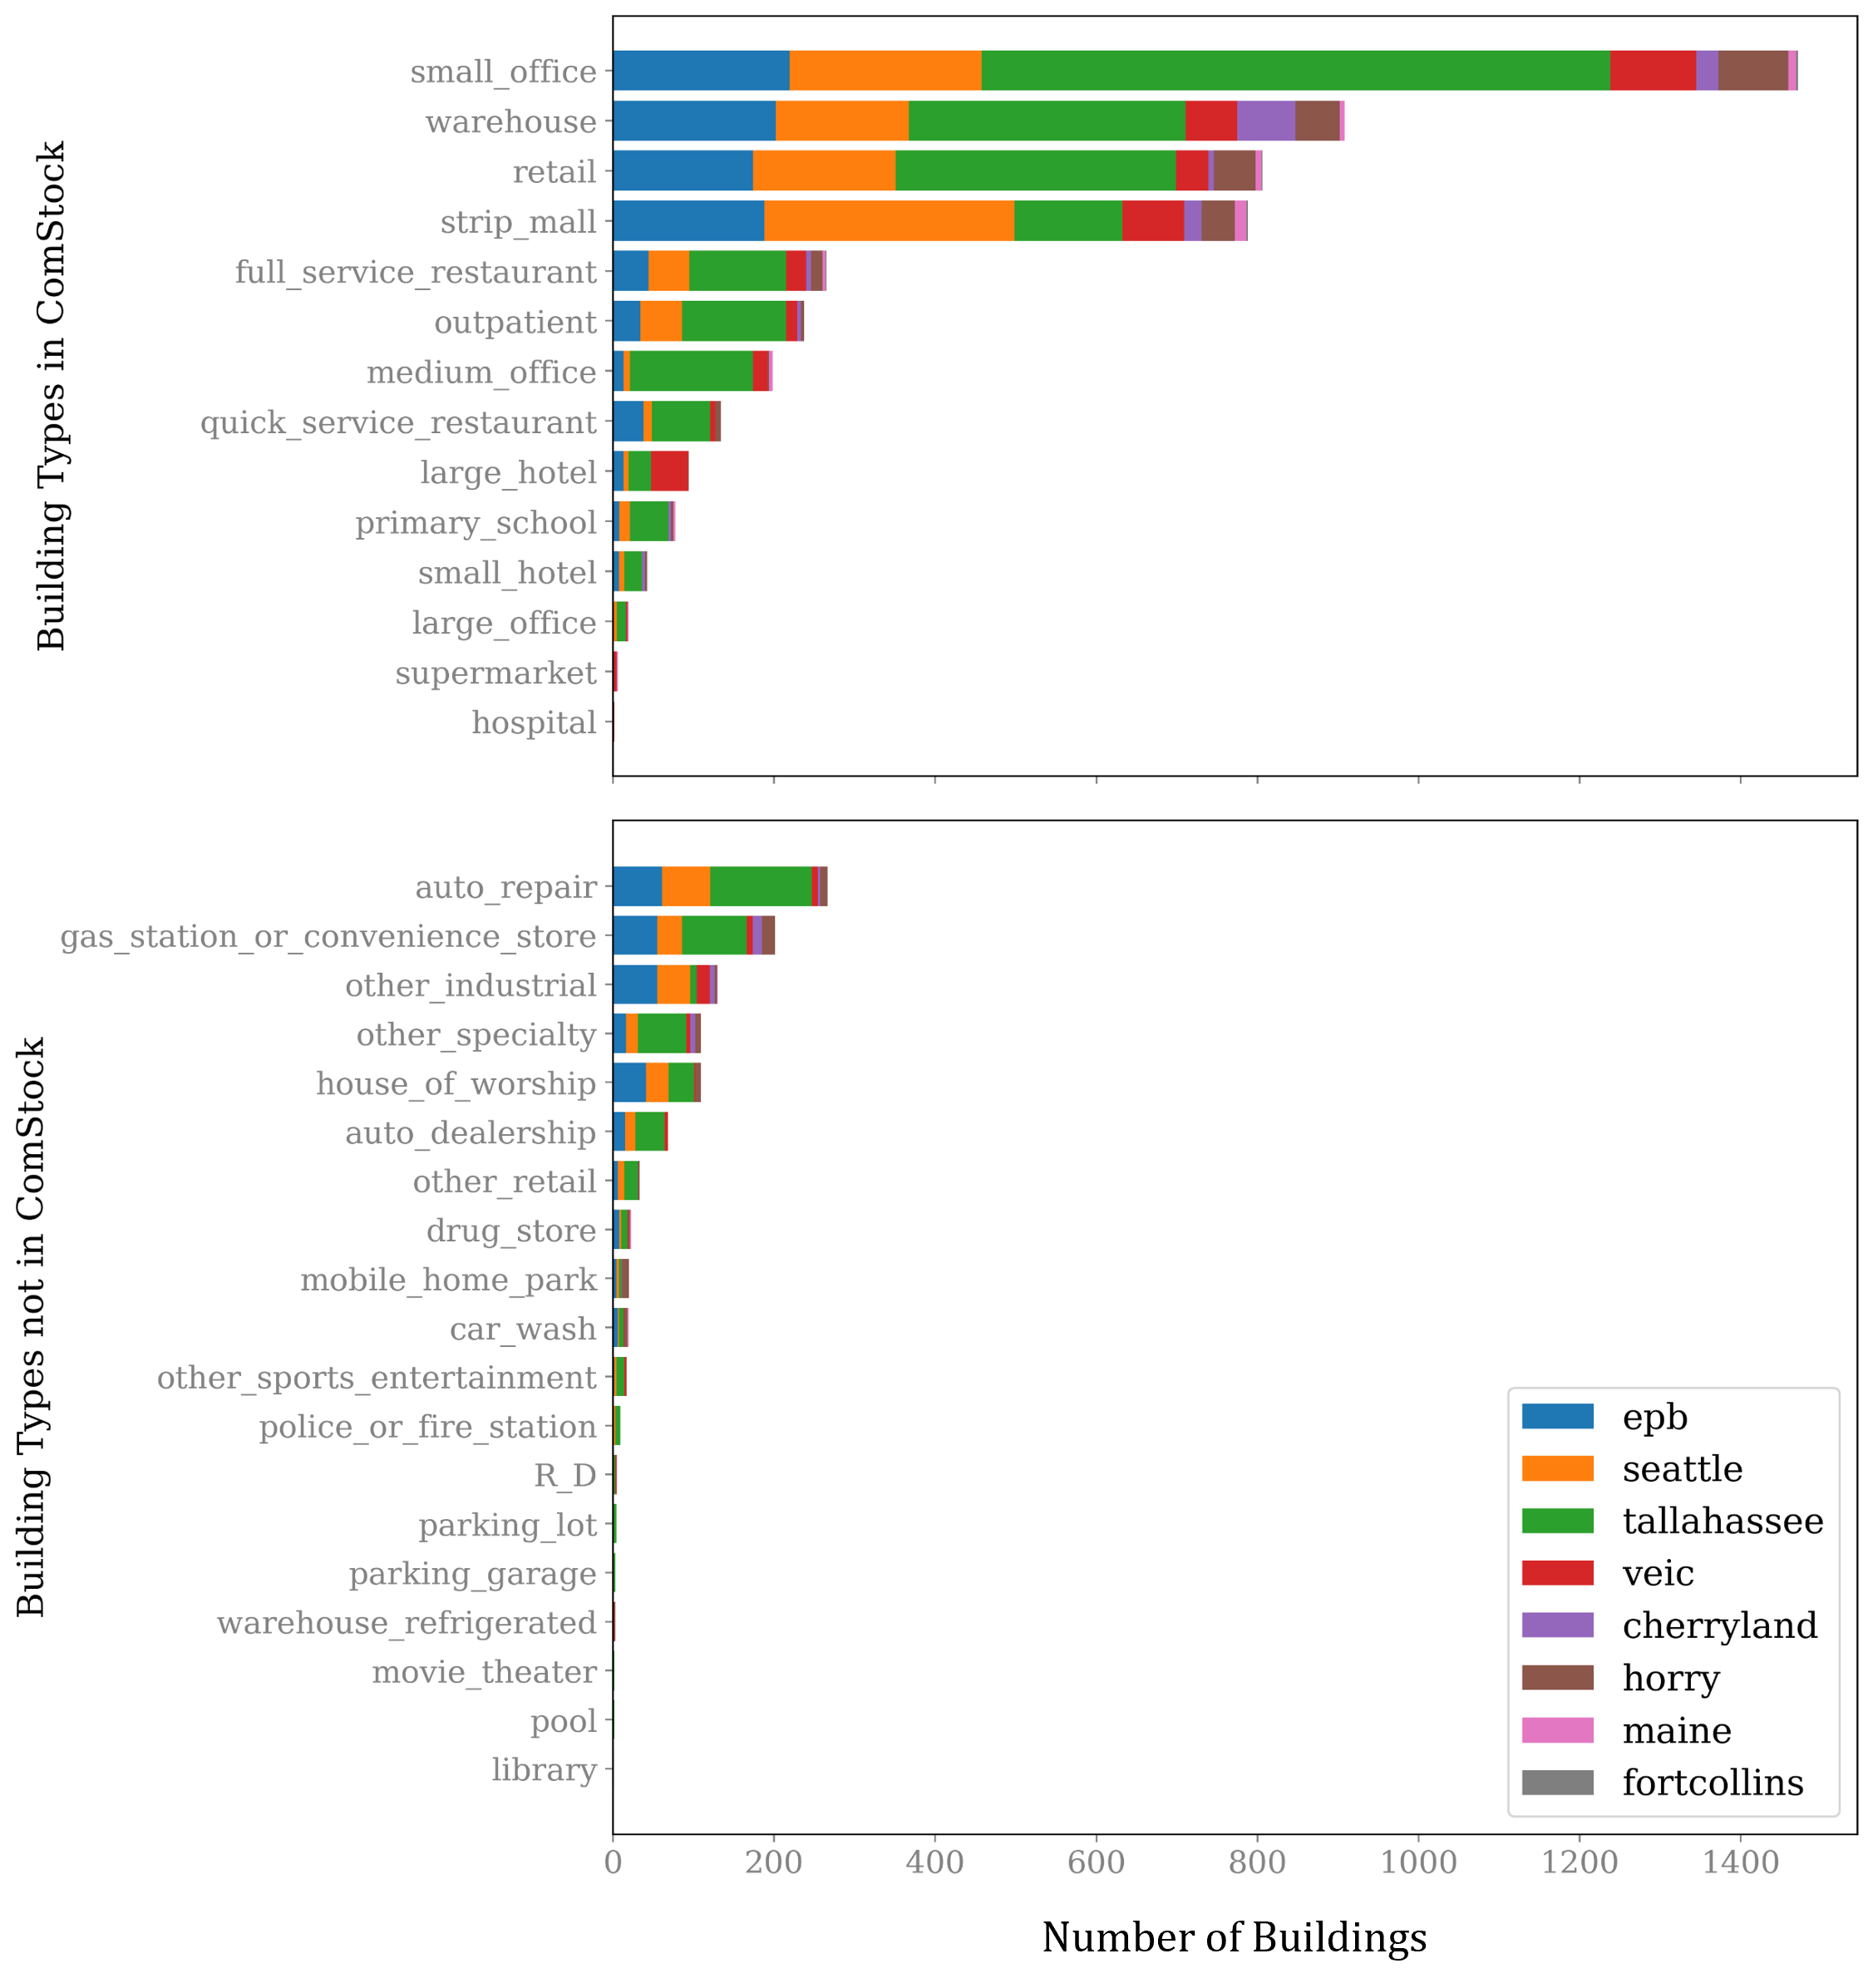
\includegraphics[width=0.8\textwidth]{figures/utility_building_type.png}
%    \caption[Number of samples by building type and utility in the commercial AMI data set]{Number of samples by building type and utility in the commercial AMI data set used to derive hours of operation schedules. See EULP Final Technical Report Table 10 for more detail.}
%    \label{fig:utility_building_type}
%\end{figure}

We compared the distribution extracted from the commercial schedules AMI data set with the inputs of ComStock at the start of the EULP calibration. The results of the small office building type are presented in Figure~\ref{fig:small_office_season} to illustrate the process, because this building type has the largest sample size in the AMI data set. We considered two day types, working day vs. non-working day, and two season definitions---one defined by month, and the other defined by daily average outdoor air temperature. The distribution of hours of operation is more diffuse in the AMI data set than in the ComStock inputs at the start of EULP calibration. Also, the duration of high load is smaller in the real AMI data than in the previous ComStock assumptions.

%\begin{figure}
%    \centering 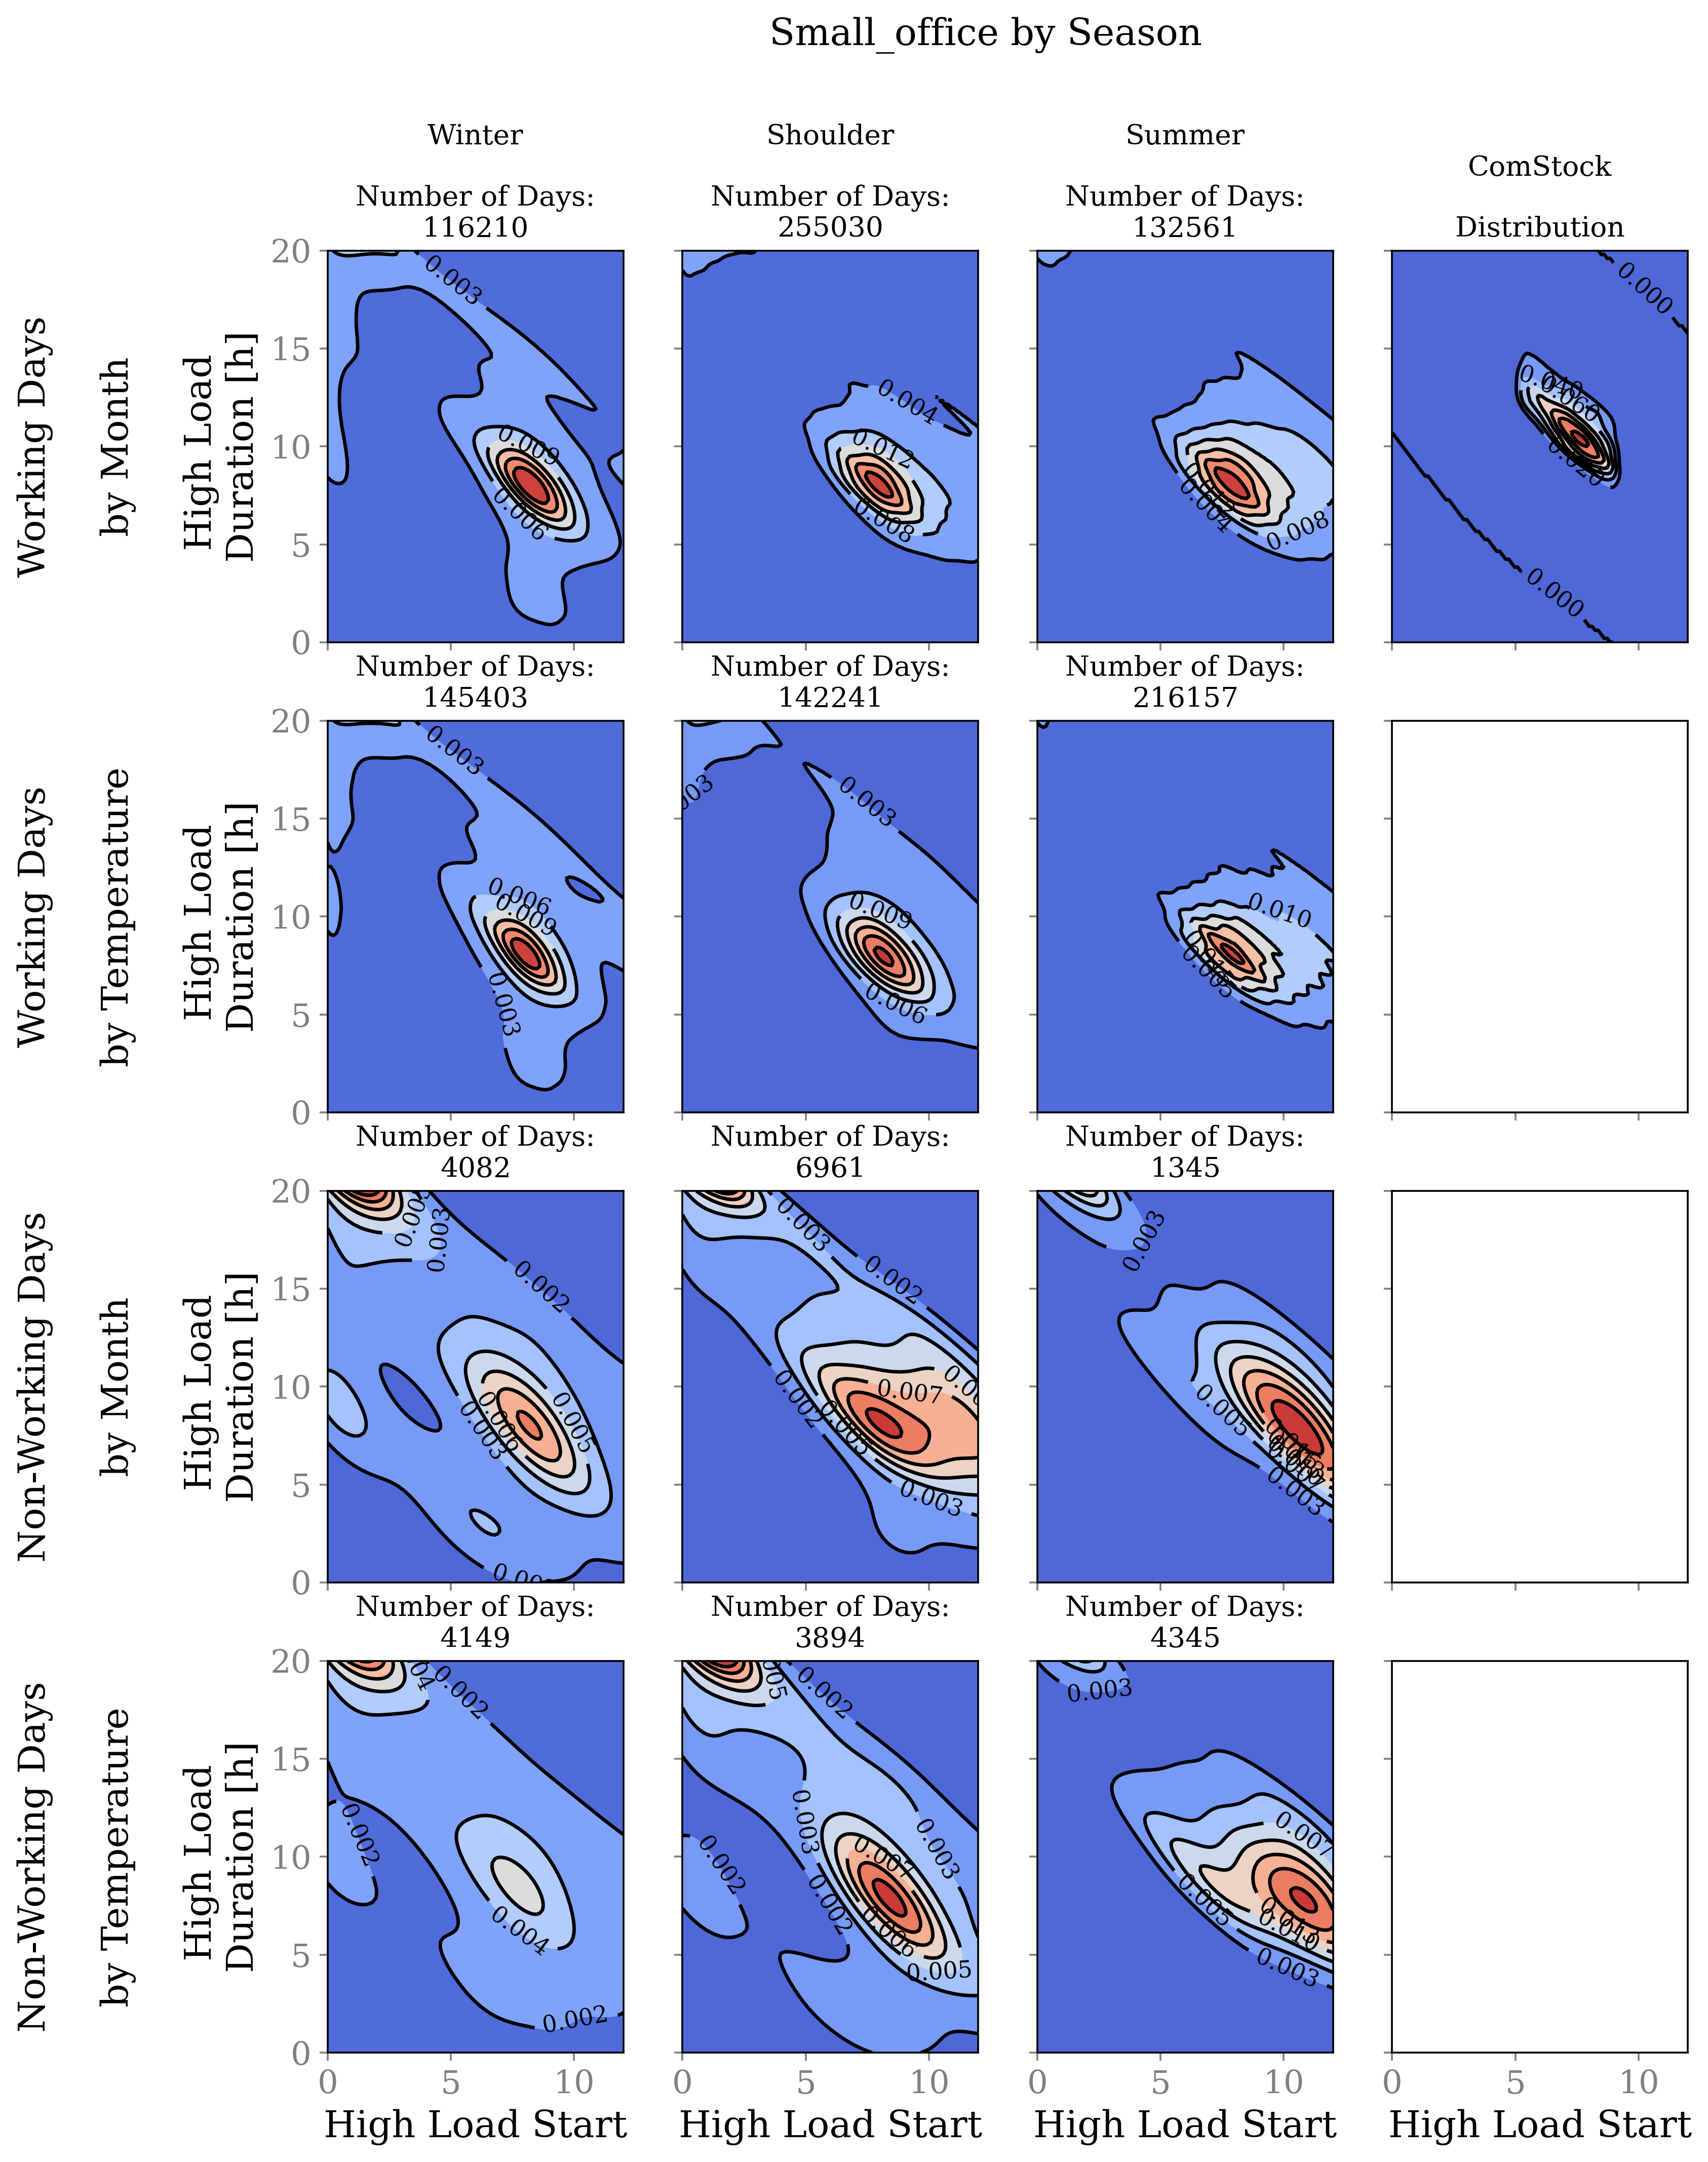
\includegraphics[width=0.8\textwidth]{figures/small_office_season.png}
%    \caption[Distribution of small office hours of operations, by day type and season]{Distribution of small office hours of operations extracted from AMI data (from seven utilities), by day type and season, and compared to ComStock before updates. This figure shows how the hours of operation (start time and duration of the high load period) are influenced by season (all utilities are combined in this plot).}
    %\label{fig:small_office_season}
%\end{figure}

%\begin{figure}
%    \centering 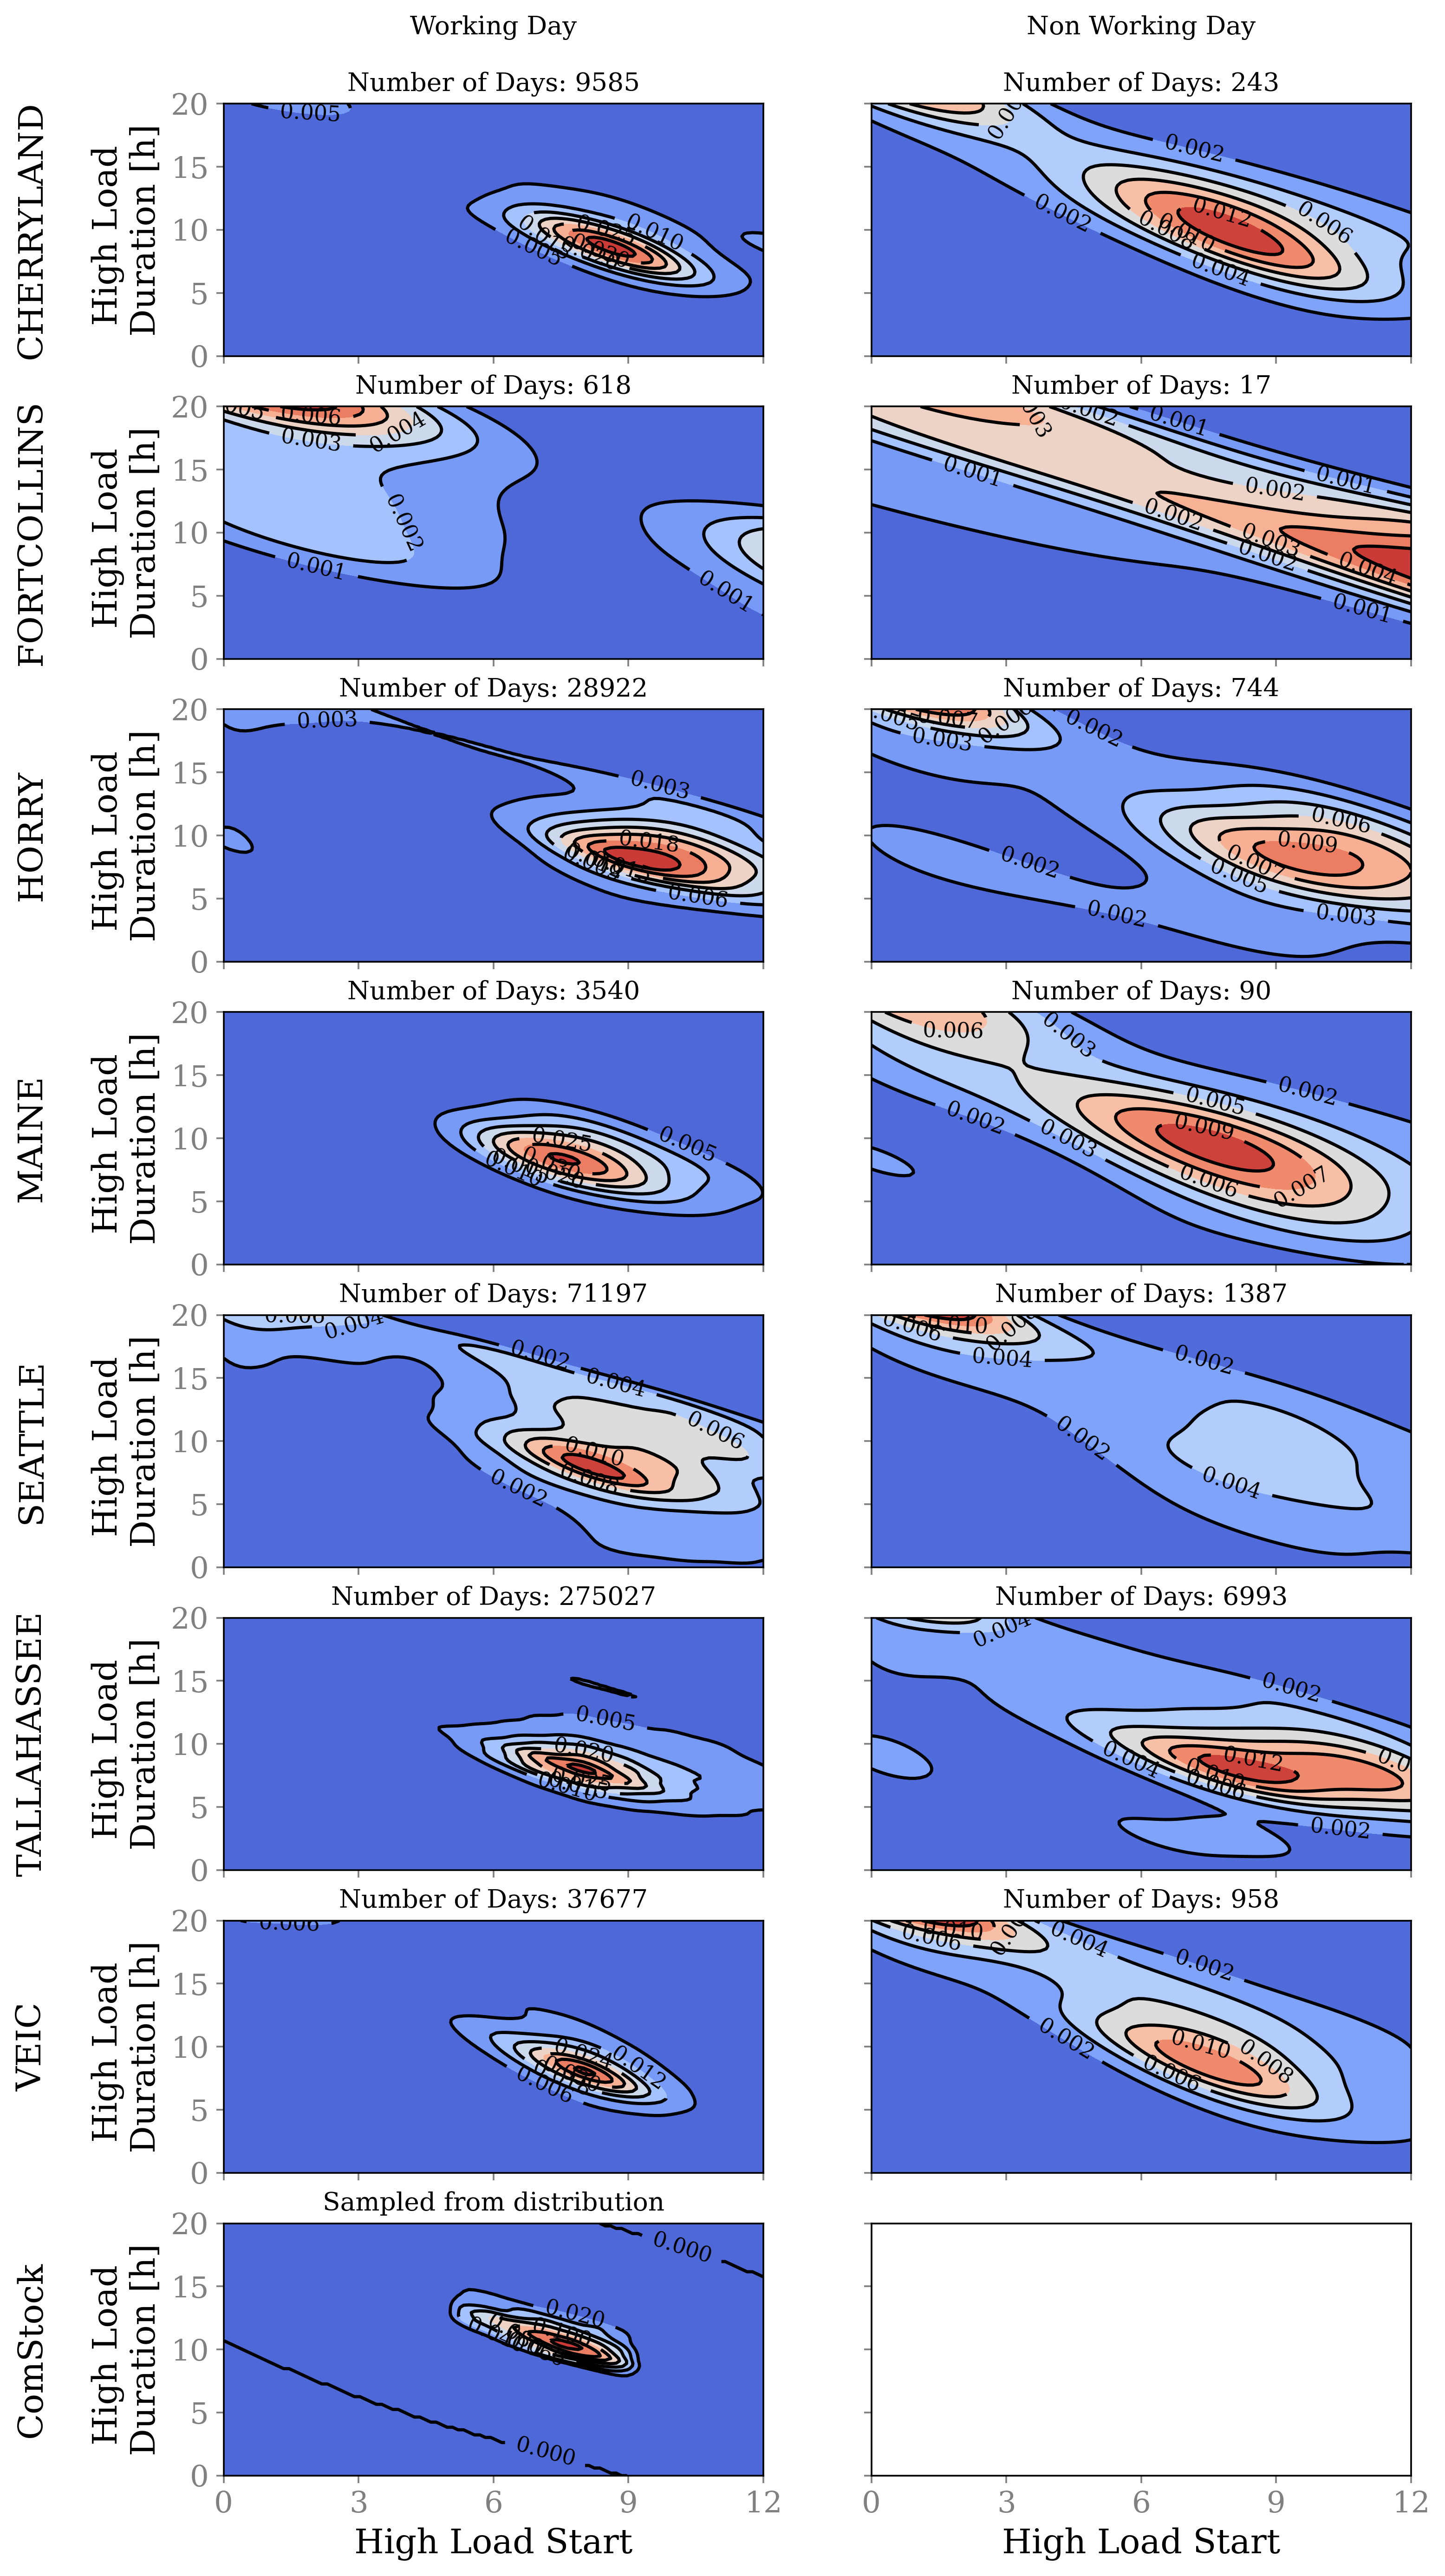
\includegraphics[width=0.7\textwidth]{figures/small_office_utility.png}
 %   \caption[Distribution of small office hours of operation, by utility and day type]{Distribution of small office hours of operations extracted from AMI data (from seven utilities), by utility and day type, and compared to ComStock before updates. This figure shows how the hours of operation (start time and duration of the high load period) are influenced by utility region (all seasons are combined in this plot).}
    %\label{fig:small_office_utility}
%   \end{figure}

We explored whether and how the hours of operation are influenced by season (in Figure~\ref{fig:small_office_season}) and by utility (in Figure \ref{fig:small_office_utility}). Some differences can be observed; however, due to the modeling complexity and the desire to create a nationally applicable approach that avoids overfitting to a specific utility region, we combined the AMI data across seasons and utilities to generate a distribution of hours of operation for each building type. These new distributions were applied to ComStock in place of the existing distributions.


\subsection{Occupancy}
\subsubsection{Occupancy Density}
Occupants are assigned to individual space types as an occupancy density (people/1000 ft\textsuperscript{2}). This value, when multiplied by the total zone floor area, determines the maximum number of people in a zone.  \Crefrange{tab:food_service_occupancy_density}{tab:warehouse_occupancy_density} show the occupancy densities for all space types included in ComStock.

The majority of the ComStock occupancy density values are from the DOE prototype models. These are derived primarily from ASHRAE 62.1-2004 \citep{ashrae_62.1_2004}, with some space type densities originating from the International Building Code 2003 \citep{icc_2003}. Prototype hotel guest rooms were assumed to have 1.5 occupants each, and occupancy rates for the two hotel models were assumed to be 65\% to align with the industry average occupancy rate and \cite{jiang_2008}. Rooms were randomly assigned occupants so that 65\% of the rooms were occupied. Most of the DOE prototype hospital and outpatient space type occupancy densities were replaced with values from the 2007 Green Guide for Healthcare (GGHC), which includes typical occupancy densities for healthcare space types \citep{gghc_2007}.

\subsubsection{Occupancy Schedules}
The maximum number of people in a zone (calculated from occupancy density and zone floor area) is multiplied by an hourly occupancy schedule with values ranging from zero to one to capture the variation in building occupancy throughout the day. Figures \ref{fig:occupancy_schedules_1} and \ref{fig:occupancy_schedules_2} show the national base occupancy schedules used in ComStock, broken down by building type. For the California occupancy schedules, please see figures \ref{fig:occupancy_schedules_deer_1} and \ref{fig:occupancy_schedules_deer_2} in the Appendix. For buildings in all states except California, the base schedules are the DOE prototype occupancy schedules. California uses schedules from DEER prototype models \citep{cpuc_deer}. The DOE prototype documentation \citep{deru_2011} notes that there are few data sources that provide operating schedules for use in building energy simulations. Thus, the schedules in the prototype models were derived from two primary data sources: the Advanced Energy Design Guide Technical Support Documents \citep{jiang_2008,doebber_2009,liu_2007,pless_2007} and ASHRAE 90.1-1989 Section 13 \citep{ashrae_1989}. These schedules were then modified to account for real-world building operation, based on the experience of the engineers who created the DOE prototype models. Classroom occupancy schedules for primary and secondary schools were adjusted by factors of 0.75 and 0.70, respectively, to meet the student numbers documented in \cite{pless_2007}. Table~\ref{tab:occupancy_schedule_source} lists the data sources for occupancy schedules in each of the prototype buildings (both DOE and DEER).

These base occupancy schedules are stretched, compressed, or shifted in time to reflect the model’s assigned hours of operation. For example, the base occupancy schedule for large offices is 9 a.m.--5 p.m. (8 hours of operation). If one large office model is assigned a start time of 8 a.m. and an operating duration of 10 hours, the base schedules in the model will be stretched so that the occupied period is an additional two hours long. All schedules in the model (occupancy, lighting, thermostat, plug load, etc.) are modified in the same manner to ensure coordination between occupancy, lighting, etc.  

%\begin{figure}
%    \centering
%    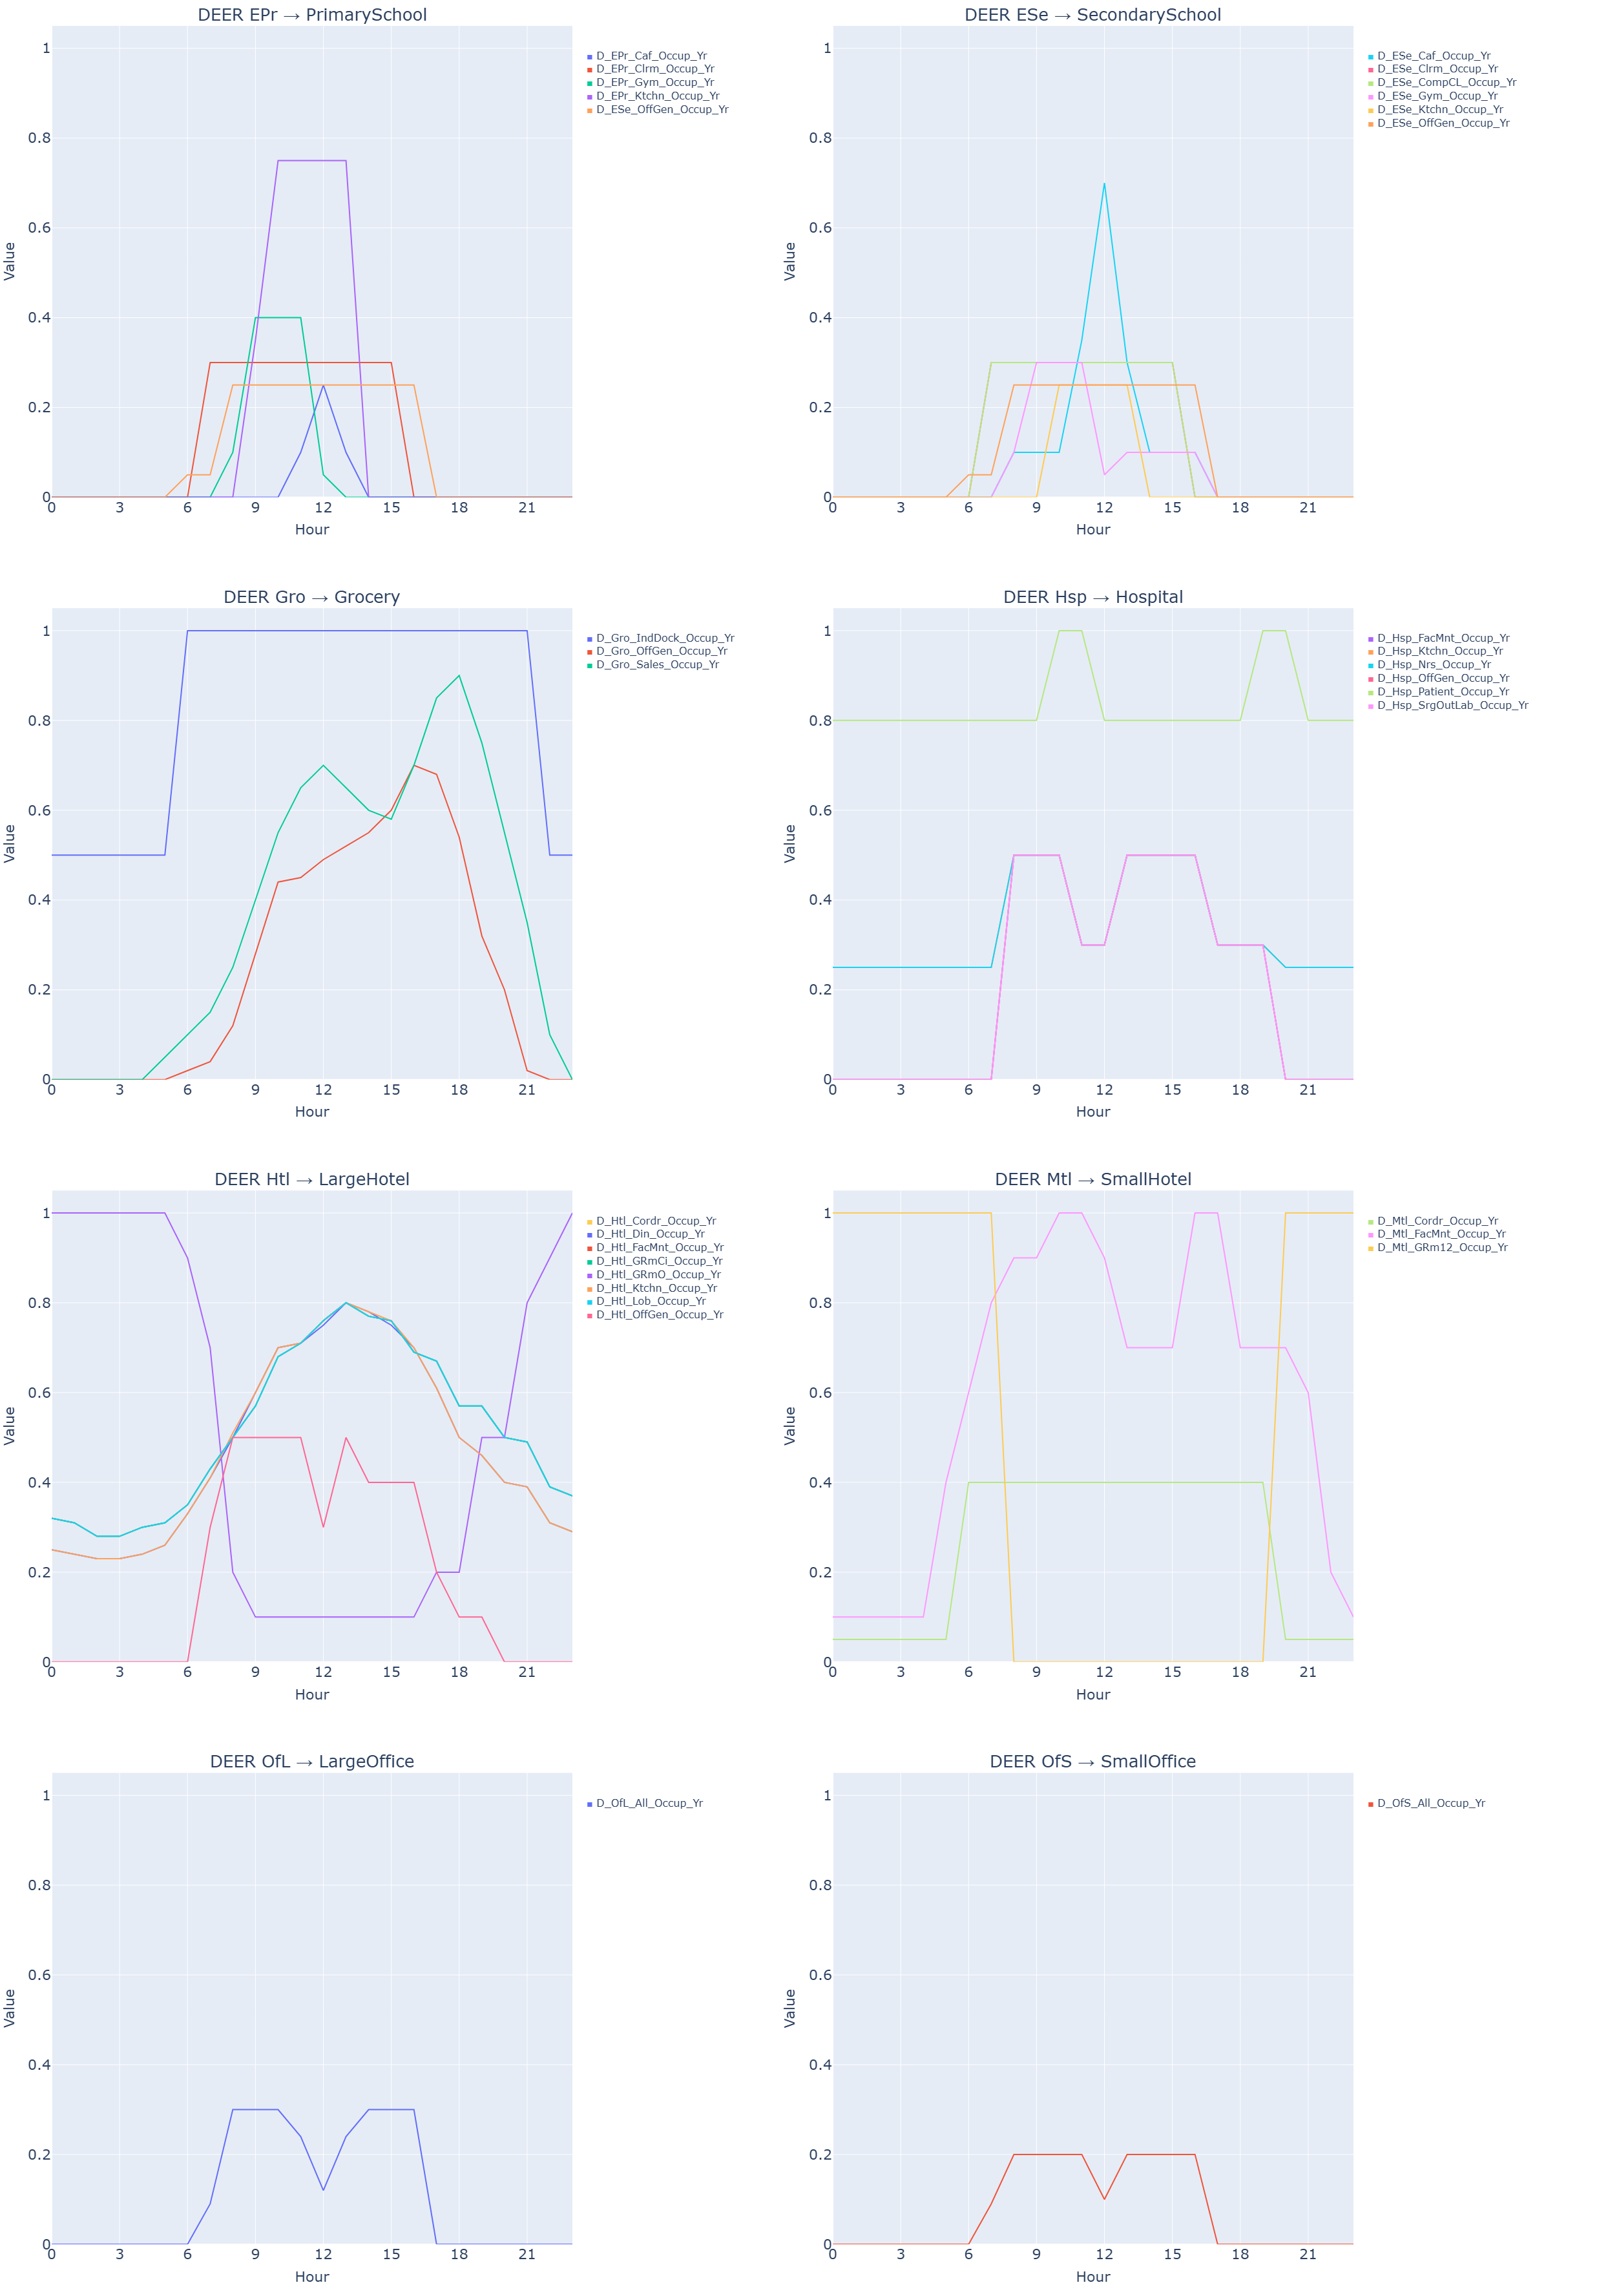
\includegraphics[trim={0 0 0 0}, clip,  % L B R T
%    width=\textwidth]{figures/occupancy_schedules_deer_1.png}
%    \caption{California base occupancy schedules for food service, lodging, healthcare, and education ComStock building types.}
%    \label{fig:occupancy_schedules_deer_1}
%\end{figure}

%\begin{figure}
%    \centering
%    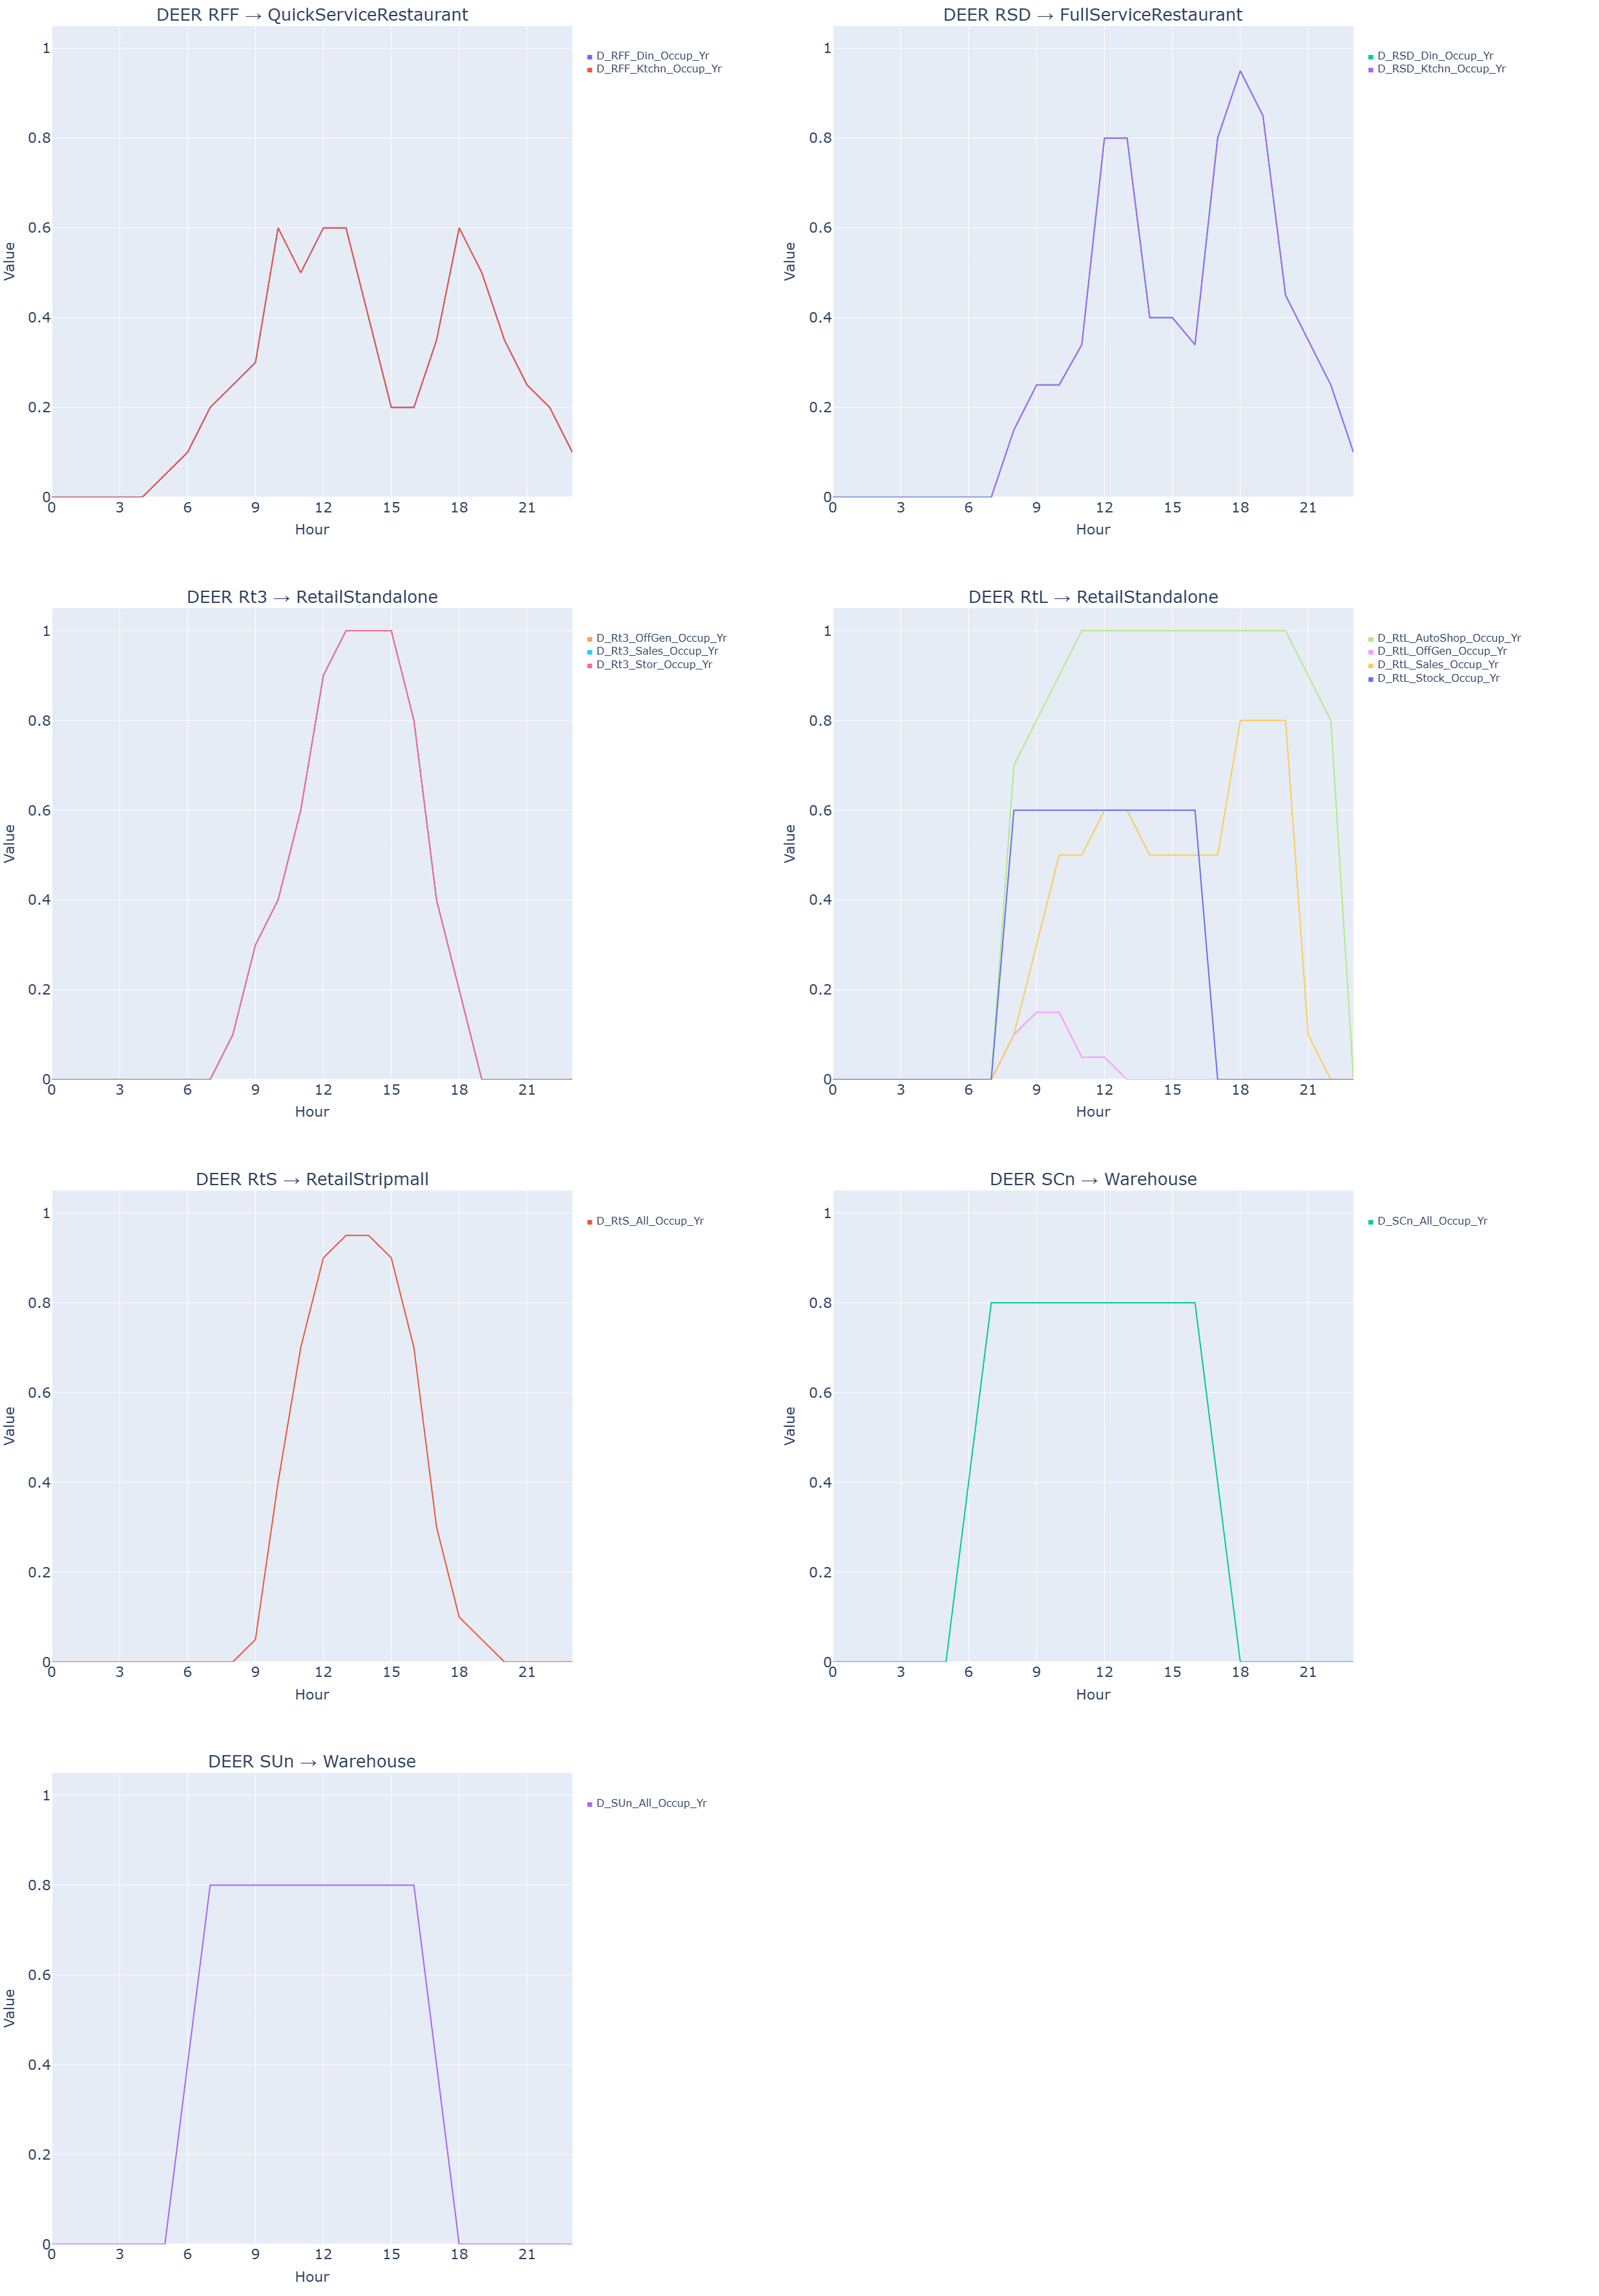
\includegraphics[trim={0 0 0 0}, clip,  % L B R T
%    width=\textwidth]{figures/occupancy_schedules_deer_2.png}
%    \caption{California base occupancy schedules for retail, office, and warehouse ComStock building types.}
 %   \label{fig:occupancy_schedules_deer_2}
%\end{figure}

\subsubsection{Occupancy Activity Schedules}
Occupancy activity schedules represent the total heat gain per person, including convective, radiant, and latent heat. An internal EnergyPlus algorithm determines the fraction of the total load that is sensible and latent. The sensible portion is further divided into radiant and convective using the default fraction radiant value. DOE prototype activity levels are fixed for a given building type and range from 120--132 watts per person across the various building types. DEER prototype activity levels vary by space type and range from 117--331 watts per person. Table~\ref{tab:activity_schedule} lists the occupancy activity schedules used in ComStock.

%\begin{table}
\small
\centering
\caption[Occupant Activity Schedules]{Occupant Activity Schedules by Building Type}
\label{tab:activity_schedule}
\begin{tabular}{|l|c|c|} 
\hline
\textbf{Schedule Name}      & \textbf{Outside CA Activity Level (W/person)} & \textbf{Inside CA Activity Level (W/person)}  \\ 
\hline
Hospital                    & 120           & 132--220                      \\ 
\hline
Large Hotel                 & 120           & 117--220                       \\ 
\hline
Small Hotel                 & 132           & 117--220                         \\ 
\hline
Outpatient                  & 120            & 117--220                   \\ 
\hline
Quick Service Restaurant    & 120           & 132--220                           \\ 
\hline
Full Service Restaurant     & 120           & 132--220                        \\ 
\hline
Retail                      & 120       & 132--220                          \\ 
\hline
Primary School              & 120       & 117--331                            \\ 
\hline
Secondary School            & 120          & 117--331                       \\ 
\hline
Warehouse                   & 131.85        & 132--220                          \\ 
\hline
Small Office                & 120        & 117--220                         \\ 
\hline
Medium Office               & 120            & 117--220                     \\ 
\hline
Large Office                & 120          & 117--220                       \\
\hline
\end{tabular}
\end{table}
\pagebreak

%\begin{table}[t]
\small
\centering
\caption[Occupant Density for Food Service]{Food Service (Full Service Restaurant and Quick Service Restaurant) Occupant Density Values by Space Type}
\label{tab:food_service_occupancy_density}
\begin{tabular}{|c|c|c|c|c|}
\hline
\textbf{Building Type} & \textbf{DOE Space Type} & \textbf{\begin{tabular}[c]{@{}c@{}}DOE Occupancy per Area\\ (people/1000 ft\textsuperscript{2})\end{tabular}} & \textbf{DEER Space Type} & \textbf{\begin{tabular}[c]{@{}c@{}}DEER Occupancy per Area\\ (people/1000 ft\textsuperscript{2})\end{tabular}} \\ \hline
QuickServiceRestaurant & Dining                  & 70                                                                                                            & Dining                   & 44.4                                                                                                           \\ \hline
QuickServiceRestaurant & Kitchen                 & 5                                                                                                             & Kitchen                  & 3.3                                                                                                            \\ \hline
QuickServiceRestaurant & Attic                   & 0                                                                                                             & StockRoom                & 2.2                                                                                                            \\ \hline
QuickServiceRestaurant & --                      & --                                                                                                            & CorridorStairway         & 6.7                                                                                                            \\ \hline
QuickServiceRestaurant & --                      & --                                                                                                            & LobbyWaiting             & 6.7                                                                                                            \\ \hline
QuickServiceRestaurant & --                      & --                                                                                                            & OfficeGeneral            & 4.4                                                                                                            \\ \hline
QuickServiceRestaurant & --                      & --                                                                                                            & Restroom                 & 19                                                                                                             \\ \hline
FullServiceRestaurant  & Dining                  & 70                                                                                                            & Dining                   & 44.4                                                                                                           \\ \hline
FullServiceRestaurant  & Kitchen                 & 5                                                                                                             & Kitchen                  & 3.3                                                                                                            \\ \hline
FullServiceRestaurant  & Attic                   & 0                                                                                                             & StockRoom                & 2.2                                                                                                            \\ \hline
FullServiceRestaurant  & --                      & --                                                                                                            & CorridorStairway         & 6.7                                                                                                            \\ \hline
FullServiceRestaurant  & --                      & --                                                                                                            & LobbyWaiting             & 6.7                                                                                                            \\ \hline
FullServiceRestaurant  & --                      & --                                                                                                            & OfficeGeneral            & 4.4                                                                                                            \\ \hline
FullServiceRestaurant  & --                      & --                                                                                                            & Restroom                 & 19                                                                                                             \\ \hline
\end{tabular}
\end{table}

%\begin{table}
\footnotesize
\centering
\caption[Occupant Density for Healthcare]{Healthcare (Hospital and Outpatient) Occupant Density Values by Space Type}
\label{tab:healthcare_occupancy_density}
\begin{tabular}{|c|c|c|c|c|}
\hline
\textbf{Building Type} & \textbf{DOE Space Type} & \textbf{\begin{tabular}[c]{@{}c@{}}DOE Occupancy per Area\\ (people/1000 ft\textsuperscript{2})\end{tabular}} & \textbf{DEER Space Type} & \textbf{\begin{tabular}[c]{@{}c@{}}DEER Occupancy per Area\\ (people/1000 ft\textsuperscript{2})\end{tabular}} \\ \hline
Hospital               & Dining                  & 10                                                                                                            & Dining                            & 44.4                                                                                                           \\ \hline
Hospital               & Basement                & 2.5                                                                                                           & FacMaint                          & 2.2                                                                                                            \\ \hline
Hospital               & Corridor                & 1                                                                                                             & \multirow{2}{*}{Hall}             & \multirow{2}{*}{6.7}                                                                                           \\ \cline{1-3}
Hospital               & PatCorridor             & 1                                                                                                             &                                   &                                                                                                                \\ \hline
Hospital               & NurseStn                & 1.333                                                                                                         & HspNursing                        & 6.7                                                                                                            \\ \hline
Hospital               & Kitchen                 & 5                                                                                                             & Kitchen                           & 3.3                                                                                                            \\ \hline
Hospital               & Lobby                   & 7.14                                                                                                          & LobbyWaiting                      & 6.7                                                                                                            \\ \hline
Hospital               & Office                  & 6.99                                                                                                          & OfficeGeneral                     & 4.4                                                                                                            \\ \hline
Hospital               & PatRoom                 & 5                                                                                                             & PatientRoom                       & 6.7                                                                                                            \\ \hline
Hospital               & ER\_Exam                & 20                                                                                                            & --                                & --                                                                                                             \\ \hline
Hospital               & ER\_NurseStn            & 1.333                                                                                                         & --                                & --                                                                                                             \\ \hline
Hospital               & ER\_Trauma              & 20                                                                                                            & --                                & --                                                                                                             \\ \hline
Hospital               & ER\_Triage              & 20                                                                                                            & --                                & --                                                                                                             \\ \hline
Hospital               & ICU\_NurseStn           & 1.333                                                                                                         & --                                & --                                                                                                             \\ \hline
Hospital               & ICU\_Open               & 5                                                                                                             & --                                & --                                                                                                             \\ \hline
Hospital               & ICU\_PatRm              & 5                                                                                                             & --                                & --                                                                                                             \\ \hline
Hospital               & OR                      & 5                                                                                                             & --                                & --                                                                                                             \\ \hline
Hospital               & PhysTherapy             & 5                                                                                                             & --                                & --                                                                                                             \\ \hline
Hospital               & Radiology               & 5                                                                                                             & --                                & --                                                                                                             \\ \hline
Hospital               & Lab                     & 5                                                                                                             & --                                & --                                                                                                             \\ \hline
Hospital               & --                      & --                                                                                                            & HspSurgOutptLab                   & 6.7                                                                                                            \\ \hline
Hospital               & --                      & --                                                                                                            & Restroom                          & 19                                                                                                             \\ \hline
Hospital               & --                      & --                                                                                                            & RetailSales                       & 22.2                                                                                                           \\ \hline
Hospital               & --                      & --                                                                                                            & StockRoom                         & 2.2                                                                                                            \\ \hline
Hospital               & --                      & --                                                                                                            & Break                             & 6.7                                                                                                            \\ \hline
Outpatient             & Conference              & 49.95                                                                                                         & Conference                        & 44.4                                                                                                           \\ \hline
Outpatient             & Hall                    & 0                                                                                                             & \multirow{2}{*}{CorridorStairway} & \multirow{2}{*}{6.7}                                                                                           \\ \cline{1-3}
Outpatient             & Stair                   & 0                                                                                                             &                                   &                                                                                                                \\ \hline
Outpatient             & Lobby                   & 10                                                                                                            & LobbyWaiting                      & 6.7                                                                                                            \\ \hline
Outpatient             & Elec/MechRoom           & 0                                                                                                             & MechElecRoom                      & 2.2                                                                                                            \\ \hline
Outpatient             & \multirow{2}{*}{Office} & \multirow{2}{*}{5}                                                                                            & OfficeOpen                        & 6.7                                                                                                            \\ \cline{1-1} \cline{4-5} 
Outpatient             &                         &                                                                                                               & OfficeSmall                       & 4.4                                                                                                            \\ \hline
Outpatient             & Toilet                  & 0                                                                                                             & Restroom                          & 19                                                                                                             \\ \hline
Outpatient             & Anesthesia              & 20.02                                                                                                         & --                                & --                                                                                                             \\ \hline
Outpatient             & BioHazard               & 0                                                                                                             & --                                & --                                                                                                             \\ \hline
Outpatient             & Cafe                    & 99.89                                                                                                         & --                                & --                                                                                                             \\ \hline
Outpatient             & CleanWork               & 20.02                                                                                                         & --                                & --                                                                                                             \\ \hline
Outpatient             & DressingRoom            & 5                                                                                                             & --                                & --                                                                                                             \\ \hline
Outpatient             & ElevatorPumpRoom        & 0                                                                                                             & --                                & --                                                                                                             \\ \hline
Outpatient             & Exam                    & 20.02                                                                                                         & --                                & --                                                                                                             \\ \hline
Outpatient             & IT\_Room                & 5                                                                                                             & --                                & --                                                                                                             \\ \hline
Outpatient             & Janitor                 & 0                                                                                                             & --                                & --                                                                                                             \\ \hline
Outpatient             & LockerRoom              & 15.01                                                                                                         & --                                & --                                                                                                             \\ \hline
Outpatient             & Lounge                  & 15.01                                                                                                         & --                                & --                                                                                                             \\ \hline
Outpatient             & MedGas                  & 0                                                                                                             & --                                & --                                                                                                             \\ \hline
Outpatient             & MRI                     & 20.02                                                                                                         & --                                & --                                                                                                             \\ \hline
Outpatient             & MRI\_Control            & 20.02                                                                                                         & --                                & --                                                                                                             \\ \hline
Outpatient             & NurseStation            & 20.02                                                                                                         & --                                & --                                                                                                             \\ \hline
Outpatient             & OR                      & 20.02                                                                                                         & --                                & --                                                                                                             \\ \hline
Outpatient             & PACU                    & 20.02                                                                                                         & --                                & --                                                                                                             \\ \hline
Outpatient             & PhysicalTherapy         & 20.02                                                                                                         & --                                & --                                                                                                             \\ \hline
Outpatient             & PreOp                   & 10                                                                                                            & --                                & --                                                                                                             \\ \hline
Outpatient             & ProcedureRoom           & 20.02                                                                                                         & --                                & --                                                                                                             \\ \hline
Outpatient             & Reception               & 29.97                                                                                                         & --                                & --                                                                                                             \\ \hline
Outpatient             & Soil Work               & 20.02                                                                                                         & --                                & --                                                                                                             \\ \hline
Outpatient             & Undeveloped             & 0                                                                                                             & --                                & --                                                                                                             \\ \hline
Outpatient             & Xray                    & 20.02                                                                                                         & --                                & --                                                                                                             \\ \hline
Outpatient             & --                      & --                                                                                                            & HspSurgOutptLab                   & 6.7                                                                                                            \\ \hline
Outpatient             & --                      & --                                                                                                            & Restroom                          & 19                                                                                                             \\ \hline
Outpatient             & --                      & --                                                                                                            & RetailSales                       & 22.2                                                                                                           \\ \hline
Outpatient             & --                      & --                                                                                                            & StockRoom                         & 2.2                                                                                                            \\ \hline
Outpatient             & --                      & --                                                                                                            & Break                             & 6.7                                                                                                            \\ \hline
Outpatient             & --                      & --                                                                                                            & CopyRoom                          & 5.3                                                                                                            \\ \hline
\end{tabular}
\end{table}
%\begin{table}
\small
\centering
\caption[Occupant Density for Hotels]{Hotel (Large Hotel and Small Hotel) Occupant Density Values by Space Type}
\label{tab:hotel_occupancy_density}
\begin{tabular}{|c|c|c|c|c|}
\hline
\textbf{Building Type} & \textbf{DOE Space Type} & \textbf{\begin{tabular}[c]{@{}c@{}}DOE Occupancy per Area\\ (people/1000 ft\textsuperscript{2})\end{tabular}} & \textbf{DEER Space Type} & \textbf{\begin{tabular}[c]{@{}c@{}}DEER Occupancy per Area\\ (people/1000 ft\textsuperscript{2})\end{tabular}} \\ \hline
LargeHotel             & Cafe                    & 67                                                                                                            & Dining                            & 44.4                                                                                                           \\ \hline
LargeHotel             & Corridor                & 1                                                                                                             & \multirow{2}{*}{GuestRmCorrid}    & \multirow{2}{*}{6.7}                                                                                           \\ \cline{1-3}
LargeHotel             & Corridor2               & 0                                                                                                             &                                   &                                                                                                                \\ \hline
LargeHotel             & GuestRoom               & 3.57                                                                                                          & \multirow{4}{*}{GuestRmOcc}       & \multirow{4}{*}{3.3}                                                                                           \\ \cline{1-3}
LargeHotel             & GuestRoom2              & 5.68                                                                                                          &                                   &                                                                                                                \\ \cline{1-3}
LargeHotel             & GuestRoom3              & 3.57                                                                                                          &                                   &                                                                                                                \\ \cline{1-3}
LargeHotel             & GuestRoom4              & 5.68                                                                                                          &                                   &                                                                                                                \\ \hline
LargeHotel             & Lobby                   & 30                                                                                                            & HotelLobby                        & 6.7                                                                                                            \\ \hline
LargeHotel             & Kitchen                 & 5                                                                                                             & Kitchen                           & 3.3                                                                                                            \\ \hline
LargeHotel             & Laundry                 & 4                                                                                                             & Laundry                           & 6.7                                                                                                            \\ \hline
LargeHotel             & Banquet                 & 67                                                                                                            & --                                & --                                                                                                             \\ \hline
LargeHotel             & Basement                & 5                                                                                                             & --                                & --                                                                                                             \\ \hline
LargeHotel             & Mechanical              & 0                                                                                                             & --                                & --                                                                                                             \\ \hline
LargeHotel             & Retail                  & 15                                                                                                            & --                                & --                                                                                                             \\ \hline
LargeHotel             & Retail2                 & 15                                                                                                            & --                                & --                                                                                                             \\ \hline
LargeHotel             & Storage                 & 2                                                                                                             & --                                & --                                                                                                             \\ \hline
LargeHotel             & --                      & --                                                                                                            & BarCasino                         & 44.4                                                                                                           \\ \hline
LargeHotel             & --                      & --                                                                                                            & GuestRmUnOcc                      & 3.3                                                                                                            \\ \hline
LargeHotel             & --                      & --                                                                                                            & OfficeGeneral                     & 4.4                                                                                                            \\ \hline
LargeHotel             & --                      & --                                                                                                            & Restroom                          & 19                                                                                                             \\ \hline
LargeHotel             & --                      & --                                                                                                            & StockRoom                         & 2.2                                                                                                            \\ \hline
SmallHotel             & StaffLounge             & 51.28                                                                                                         & Break                             & 6.7                                                                                                            \\ \hline
SmallHotel             & Corridor                & 0                                                                                                             & \multirow{2}{*}{GuestRmCorrid}    & \multirow{2}{*}{6.7}                                                                                           \\ \cline{1-3}
SmallHotel             & Corridor4               & 0                                                                                                             &                                   &                                                                                                                \\ \hline
SmallHotel             & Stair                   & 0                                                                                                             & \multirow{2}{*}{CorridorStairway} & \multirow{2}{*}{6.7}                                                                                           \\ \cline{1-3}
SmallHotel             & Stair4                  & 0                                                                                                             &                                   &                                                                                                                \\ \hline
SmallHotel             & GuestRoom123Occ         & 4.27                                                                                                          & \multirow{2}{*}{GuestRmOcc}       & \multirow{2}{*}{3.3}                                                                                           \\ \cline{1-3}
SmallHotel             & GuestRoom4Occ           & 4.27                                                                                                          &                                   &                                                                                                                \\ \hline
SmallHotel             & GuestRoom123Vac         & 4.27                                                                                                          & \multirow{2}{*}{GuestRmUnOcc}     & \multirow{2}{*}{3.3}                                                                                           \\ \cline{1-3}
SmallHotel             & GuestRoom4Vac           & 4.27                                                                                                          &                                   &                                                                                                                \\ \hline
SmallHotel             & Laundry                 & 10                                                                                                            & Laundry                           & 6.7                                                                                                            \\ \hline
SmallHotel             & Elec/MechRoom           & 0                                                                                                             & \multirow{2}{*}{MechElecRoom}     & \multirow{2}{*}{2.2}                                                                                           \\ \cline{1-3}
SmallHotel             & Mechanical              & 0                                                                                                             &                                   &                                                                                                                \\ \hline
SmallHotel             & Office                  & 7.14                                                                                                          & OfficeGeneral                     & 4.4                                                                                                            \\ \hline
SmallHotel             & Meeting                 & 50                                                                                                            & --                                & --                                                                                                             \\ \hline
SmallHotel             & PublicRestroom          & 2.85                                                                                                          & Restroom                          & 19                                                                                                             \\ \hline
SmallHotel             & Storage                 & 0                                                                                                             & StorageSmlCond                    & 2.2                                                                                                            \\ \hline
SmallHotel             & GuestLounge             & 30                                                                                                            & --                                & --                                                                                                             \\ \hline
SmallHotel             & ElevatorCore            & 0                                                                                                             & --                                & --                                                                                                             \\ \hline
SmallHotel             & ElevatorCore4           & 0                                                                                                             & --                                & --                                                                                                             \\ \hline
SmallHotel             & Exercise                & 19.94                                                                                                         & --                                & --                                                                                                             \\ \hline
\end{tabular}
\end{table}
%\begin{table}
\footnotesize
\centering
\caption[Occupant Density for Offices]{Office (Small Office, Medium Office, and Large Office) Occupant Density Values by Space Type}
\label{tab:office_occupancy_density}
\begin{tabular}{|c|c|c|c|c|}
\hline
\textbf{Building Type} & \textbf{DOE Space Type} & \textbf{\begin{tabular}[c]{@{}c@{}}DOE Occupancy per Area\\ (people/1000 ft\textsuperscript{2})\end{tabular}} & \textbf{DEER Space Type} & \textbf{\begin{tabular}[c]{@{}c@{}}DEER Occupancy per Area\\ (people/1000 ft\textsuperscript{2})\end{tabular}} \\ \hline
LargeOffice            & BreakRoom                    & 50                                                                                                            & Break                             & 6.7                                                                                                            \\ \hline
LargeOffice            & Conference                   & 50                                                                                                            & Conference                        & 44.4                                                                                                           \\ \hline
LargeOffice            & PrintRoom                    & 10                                                                                                            & CopyRoom                          & 5.3                                                                                                            \\ \hline
LargeOffice            & Stair                        & 0                                                                                                             & \multirow{2}{*}{CorridorStairway} & \multirow{2}{*}{6.7}                                                                                           \\ \cline{1-3}
LargeOffice            & Corridor                     & 1                                                                                                             &                                   &                                                                                                                \\ \hline
LargeOffice            & Lobby                        & 10                                                                                                            & LobbyWaiting                      & 6.7                                                                                                            \\ \hline
LargeOffice            & Elec/MechRoom                & 0                                                                                                             & MechElecRoom                      & 2.2                                                                                                            \\ \hline
LargeOffice            & OpenOffice                   & 5.25                                                                                                          & OfficeOpen                        & 6.7                                                                                                            \\ \hline
LargeOffice            & ClosedOffice                 & 4.75                                                                                                          & OfficeSmall                       & 4.4                                                                                                            \\ \hline
LargeOffice            & Restroom                     & 10                                                                                                            & Restroom                          & 19                                                                                                             \\ \hline
LargeOffice            & Storage                      & 0                                                                                                             & StorageSmlCond                    & 2.2                                                                                                            \\ \hline
LargeOffice            & WholeBuilding - Lg Office    & 5                                                                                                             & --                                & --                                                                                                             \\ \hline
LargeOffice            & Vending                      & 1                                                                                                             & --                                & --                                                                                                             \\ \hline
LargeOffice            & IT\_Room                     & 5                                                                                                             & --                                & --                                                                                                             \\ \hline
LargeOffice            & Dining                       & 10                                                                                                            & --                                & --                                                                                                             \\ \hline
LargeOffice            & Classroom                    & 35                                                                                                            & --                                & --                                                                                                             \\ \hline
MediumOffice           & MediumOffice - Breakroom     & 50                                                                                                            & Break                             & 6.7                                                                                                            \\ \hline
MediumOffice           & MediumOffice - Conference    & 50                                                                                                            & Conference                        & 44.4                                                                                                           \\ \hline
MediumOffice           & MediumOffice - Stair         & 0                                                                                                             & \multirow{2}{*}{CorridorStairway} & \multirow{2}{*}{6.7}                                                                                           \\ \cline{1-3}
MediumOffice           & MediumOffice - Corridor      & 0                                                                                                             &                                   &                                                                                                                \\ \hline
MediumOffice           & MediumOffice - Lobby         & 10                                                                                                            & LobbyWaiting                      & 6.7                                                                                                            \\ \hline
MediumOffice           & MediumOffice - Elec/MechRoom & 0                                                                                                             & MechElecRoom                      & 2.2                                                                                                            \\ \hline
MediumOffice           & MediumOffice - OpenOffice    & 5.25                                                                                                          & OfficeOpen                        & 6.7                                                                                                            \\ \hline
MediumOffice           & MediumOffice - ClosedOffice  & 4.75                                                                                                          & OfficeSmall                       & 4.4                                                                                                            \\ \hline
MediumOffice           & MediumOffice - Restroom      & 0                                                                                                             & Restroom                          & 19                                                                                                             \\ \hline
MediumOffice           & MediumOffice - Storage       & 0                                                                                                             & StorageSmlCond                    & 2.2                                                                                                            \\ \hline
MediumOffice           & MediumOffice - Dining        & 10                                                                                                            & --                                & --                                                                                                             \\ \hline
MediumOffice           & MediumOffice - Classroom     & 35                                                                                                            & --                                & --                                                                                                             \\ \hline
MediumOffice           & WholeBuilding - Md Office    & 5                                                                                                             & --                                & --                                                                                                             \\ \hline
MediumOffice           & --                           & --                                                                                                            & CopyRoom                          & 5.3                                                                                                            \\ \hline
SmallOffice            & SmallOffice - Breakroom      & 50                                                                                                            & Break                             & 6.7                                                                                                            \\ \hline
SmallOffice            & SmallOffice - Conference     & 50                                                                                                            & Conference                        & 44.4                                                                                                           \\ \hline
SmallOffice            & SmallOffice - Stair          & 0                                                                                                             & \multirow{2}{*}{Hall}             & \multirow{2}{*}{6.7}                                                                                           \\ \cline{1-3}
SmallOffice            & SmallOffice - Corridor       & 0                                                                                                             &                                   &                                                                                                                \\ \hline
SmallOffice            & SmallOffice - Lobby          & 10                                                                                                            & LobbyWaiting                      & 6.7                                                                                                            \\ \hline
SmallOffice            & SmallOffice - Elec/MechRoom  & 0                                                                                                             & MechElecRoom                      & 2.2                                                                                                            \\ \hline
SmallOffice            & SmallOffice - OpenOffice     & 5.25                                                                                                          & OfficeOpen                        & 6.7                                                                                                            \\ \hline
SmallOffice            & SmallOffice - ClosedOffice   & 4.75                                                                                                          & OfficeSmall                       & 4.4                                                                                                            \\ \hline
SmallOffice            & SmallOffice - Restroom       & 0                                                                                                             & Restroom                          & 19                                                                                                             \\ \hline
SmallOffice            & SmallOffice - Storage        & 0                                                                                                             & StorageSmlCond                    & 2.2                                                                                                            \\ \hline
SmallOffice            & SmallOffice - Dining         & 10                                                                                                            & --                                & --                                                                                                             \\ \hline
SmallOffice            & SmallOffice - Classroom      & 35                                                                                                            & --                                & --                                                                                                             \\ \hline
SmallOffice            & WholeBuilding - Sm Office    & 5.6                                                                                                           & --                                & --                                                                                                             \\ \hline
SmallOffice            & --                           & --                                                                                                            & CompRoomData                      & 6.7                                                                                                            \\ \hline
SmallOffice            & --                           & --                                                                                                            & CopyRoom                          & 5.3                                                                                                            \\ \hline
\end{tabular}
\end{table}
%\begin{table}
\small
\centering
\caption[Occupant Density for Schools]{School (Primary School and Secondary School) Occupant Density Values by Space Type}
\label{tab:school_occupancy_density}
\begin{tabular}{|c|c|c|c|c|}
\hline
\textbf{Building Type} & \textbf{DOE Space Type} & \textbf{\begin{tabular}[c]{@{}c@{}}DOE Occupancy per Area\\ (people/1000 ft\textsuperscript{2})\end{tabular}} & \textbf{DEER Space Type} & \textbf{\begin{tabular}[c]{@{}c@{}}DEER Occupancy per Area\\ (people/1000 ft\textsuperscript{2})\end{tabular}} \\ \hline
SecondarySchool        & Classroom               & 35                                                                                                            & Classroom                & 33.3                                                                                                           \\ \hline
SecondarySchool        & ComputerRoom            & 35                                                                                                            & CompRoomClassRm          & 13.3                                                                                                           \\ \hline
SecondarySchool        & Auditorium              & 150                                                                                                           & Conference               & 44.4                                                                                                           \\ \hline
SecondarySchool        & Corridor                & 0                                                                                                             & CorridorStairway         & 6.7                                                                                                            \\ \hline
SecondarySchool        & Cafeteria               & 100                                                                                                           & Dining                   & 44.4                                                                                                           \\ \hline
SecondarySchool        & Gym                     & 30                                                                                                            & Gymnasium                & 13.3                                                                                                           \\ \hline
SecondarySchool        & Kitchen                 & 15.23                                                                                                         & Kitchen                  & 3.3                                                                                                            \\ \hline
SecondarySchool        & Library                 & 10                                                                                                            & LibraryReading           & 13.3                                                                                                           \\ \hline
SecondarySchool        & Mechanical              & 0                                                                                                             & MechElecRoom             & 2.2                                                                                                            \\ \hline
SecondarySchool        & Office                  & 5                                                                                                             & OfficeGeneral            & 4.4                                                                                                            \\ \hline
SecondarySchool        & Restroom                & 0                                                                                                             & Restroom                 & 19                                                                                                             \\ \hline
SecondarySchool        & Lobby                   & 0                                                                                                             & --                       & --                                                                                                             \\ \hline
SecondarySchool        & --                      & --                                                                                                            & Shop                     & 6.7                                                                                                            \\ \hline
SecondarySchool        & --                      & --                                                                                                            & StorageSmlCond           & 2.2                                                                                                            \\ \hline
PrimarySchool          & Classroom               & 25                                                                                                            & Classroom                & 33.3                                                                                                           \\ \hline
PrimarySchool          & ComputerRoom            & 25                                                                                                            & CompRoomClassRm          & 13.3                                                                                                           \\ \hline
PrimarySchool          & Corridor                & 0                                                                                                             & CorridorStairway         & 6.7                                                                                                            \\ \hline
PrimarySchool          & Cafeteria               & 100                                                                                                           & Dining                   & 44.4                                                                                                           \\ \hline
PrimarySchool          & Gym                     & 30                                                                                                            & Gymnasium                & 13.3                                                                                                           \\ \hline
PrimarySchool          & Kitchen                 & 13.93                                                                                                         & Kitchen                  & 3.3                                                                                                            \\ \hline
PrimarySchool          & Library                 & 10                                                                                                            & LibraryReading           & 13.3                                                                                                           \\ \hline
PrimarySchool          & Lobby                   & 0                                                                                                             & Lobby                    & 6.7                                                                                                            \\ \hline
PrimarySchool          & Office                  & 5                                                                                                             & OfficeGeneral            & 4.4                                                                                                            \\ \hline
PrimarySchool          & Restroom                & 0                                                                                                             & Restroom                 & 19                                                                                                             \\ \hline
PrimarySchool          & --                      & --                                                                                                            & StorageSmlCond           & 2.2                                                                                                            \\ \hline
\end{tabular}
\end{table}
%\begin{table}
\small
\centering
\caption[Occupant Density for Retail]{Retail (Retail and Strip Mall) Occupant Density Values by Space Type}
\label{tab:retail_occupancy_density}
\begin{tabular}{|c|c|c|c|c|}
\hline
\textbf{Building Type} & \textbf{DOE Space Type} & \textbf{\begin{tabular}[c]{@{}c@{}}DOE Occupancy per Area\\ (people/1000 ft\textsuperscript{2})\end{tabular}} & \textbf{DEER Space Type} & \textbf{\begin{tabular}[c]{@{}c@{}}DEER Occupancy per Area\\ (people/1000 ft\textsuperscript{2})\end{tabular}} \\ \hline
Retail                 & Retail                  & 15                                                                                                            & \multirow{2}{*}{RetailSales} & \multirow{2}{*}{22.2}                                                                                          \\ \cline{1-3}
Retail                 & Point\_of\_Sale         & 15                                                                                                            &                              &                                                                                                                \\ \hline
Retail                 & Back\_Space             & 15                                                                                                            & StockRoom                    & 2.2                                                                                                            \\ \hline
Retail                 & Entry                   & 15                                                                                                            & --                           & --                                                                                                             \\ \hline
Retail                 & --                      & --                                                                                                            & Break                        & 6.7                                                                                                            \\ \hline
Retail                 & --                      & --                                                                                                            & Kitchen                      & 3.3                                                                                                            \\ \hline
Retail                 & --                      & --                                                                                                            & MechElecRoom                 & 2.2                                                                                                            \\ \hline
Retail                 & --                      & --                                                                                                            & OfficeGeneral                & 4.4                                                                                                            \\ \hline
Retail                 & --                      & --                                                                                                            & Restroom                     & 19                                                                                                             \\ \hline
Retail                 & --                      & --                                                                                                            & Work                         & 6.7                                                                                                            \\ \hline
StripMall              & Strip mall - type 1     & 8                                                                                                             & \multirow{3}{*}{RetailSales} & \multirow{3}{*}{22.2}                                                                                          \\ \cline{1-3}
StripMall              & Strip mall - type 2     & 8                                                                                                             &                              &                                                                                                                \\ \cline{1-3}
StripMall              & Strip mall - type 3     & 8                                                                                                             &                              &                                                                                                                \\ \hline
StripMall              & --                      & --                                                                                                            & Break                        & 6.7                                                                                                            \\ \hline
StripMall              & --                      & --                                                                                                            & Hall                         & 6.7                                                                                                            \\ \hline
StripMall              & --                      & --                                                                                                            & MechElecRoom                 & 2.2                                                                                                            \\ \hline
StripMall              & --                      & --                                                                                                            & OfficeGeneral                & 4.4                                                                                                            \\ \hline
StripMall              & --                      & --                                                                                                            & Restroom                     & 19                                                                                                             \\ \hline
StripMall              & --                      & --                                                                                                            & StockRoom                    & 2.2                                                                                                            \\ \hline
\end{tabular}
\end{table}
%\begin{table}
\small
\centering
\caption[Occupant Density for Warehouses]{Warehouse Occupant Density Values by Space Type}
\label{tab:warehouse_occupancy_density}
\begin{tabular}{|c|c|c|c|c|}
\hline
\textbf{Building Type} & \textbf{DOE Space Type} & \textbf{\begin{tabular}[c]{@{}c@{}}DOE Occupancy per Area\\ (people/1000 ft\textsuperscript{2})\end{tabular}} & \textbf{DEER Space Type} & \textbf{\begin{tabular}[c]{@{}c@{}}DEER Occupancy per Area\\ (people/1000 ft\textsuperscript{2})\end{tabular}} \\ \hline
Warehouse              & Office                  & 1.96                                                                                                          & OfficeGeneral                    & 4.4                                                                                                            \\ \hline
Warehouse              & Fine                    & 0                                                                                                             & \multirow{2}{*}{WarehouseUnCond} & \multirow{2}{*}{2.2}                                                                                           \\ \cline{1-3}
Warehouse              & Bulk                    & 0                                                                                                             &                                  &                                                                                                                \\ \hline
Warehouse              & --                      & --                                                                                                            & Restroom                         & 19                                                                                                             \\ \hline
\end{tabular}
\end{table}

%\begin{table}
\small
\centering
\caption{Occupancy Schedule Data Sources}
\label{tab:occupancy_schedule_source}
\begin{tabular}{|l|l|l|} 
\hline
\textbf{Building Type}   & \textbf{DOE Data Source} & \textbf{DEER Data Source}  \\ 
\hline
Small Office             & \cite{ashrae_1989}    & \cite{cpuc_deer}       \\ 
\hline
Medium Office            & \cite{ashrae_1989}  & \cite{cpuc_deer}           \\ 
\hline
Large Office             & \cite{ashrae_1989}    & \cite{cpuc_deer}        \\ 
\hline
Primary School           & \cite{pless_2007}   & \cite{cpuc_deer}  \\ 
\hline
Secondary School         & \cite{pless_2007}  & \cite{cpuc_deer}   \\ 
\hline
Quick Service Restaurant & \cite{ashrae_1989} & \cite{cpuc_deer}          \\ 
\hline
Full Service Restaurant  & \cite{ashrae_1989} & \cite{cpuc_deer}        \\ 
\hline
Small Hotel              & \cite{jiang_2008}  & \cite{cpuc_deer}   \\ 
\hline
Large Hotel              & \cite{jiang_2008}  & \cite{cpuc_deer}   \\ 
\hline
Hospital                 & \cite{doebber_2009}  & \cite{cpuc_deer} \\ 
\hline
Outpatient               & \cite{doebber_2009}  & \cite{cpuc_deer} \\ 
\hline
Warehouse                & \cite{liu_2007}     & \cite{cpuc_deer}  \\ 
\hline
Retail                   & \cite{ashrae_1989}   & \cite{cpuc_deer}        \\ 
\hline
Strip Mall               & \cite{ashrae_1989}   & \cite{cpuc_deer}        \\
\hline
\end{tabular}
\end{table}
\begin{figure}
   \centering 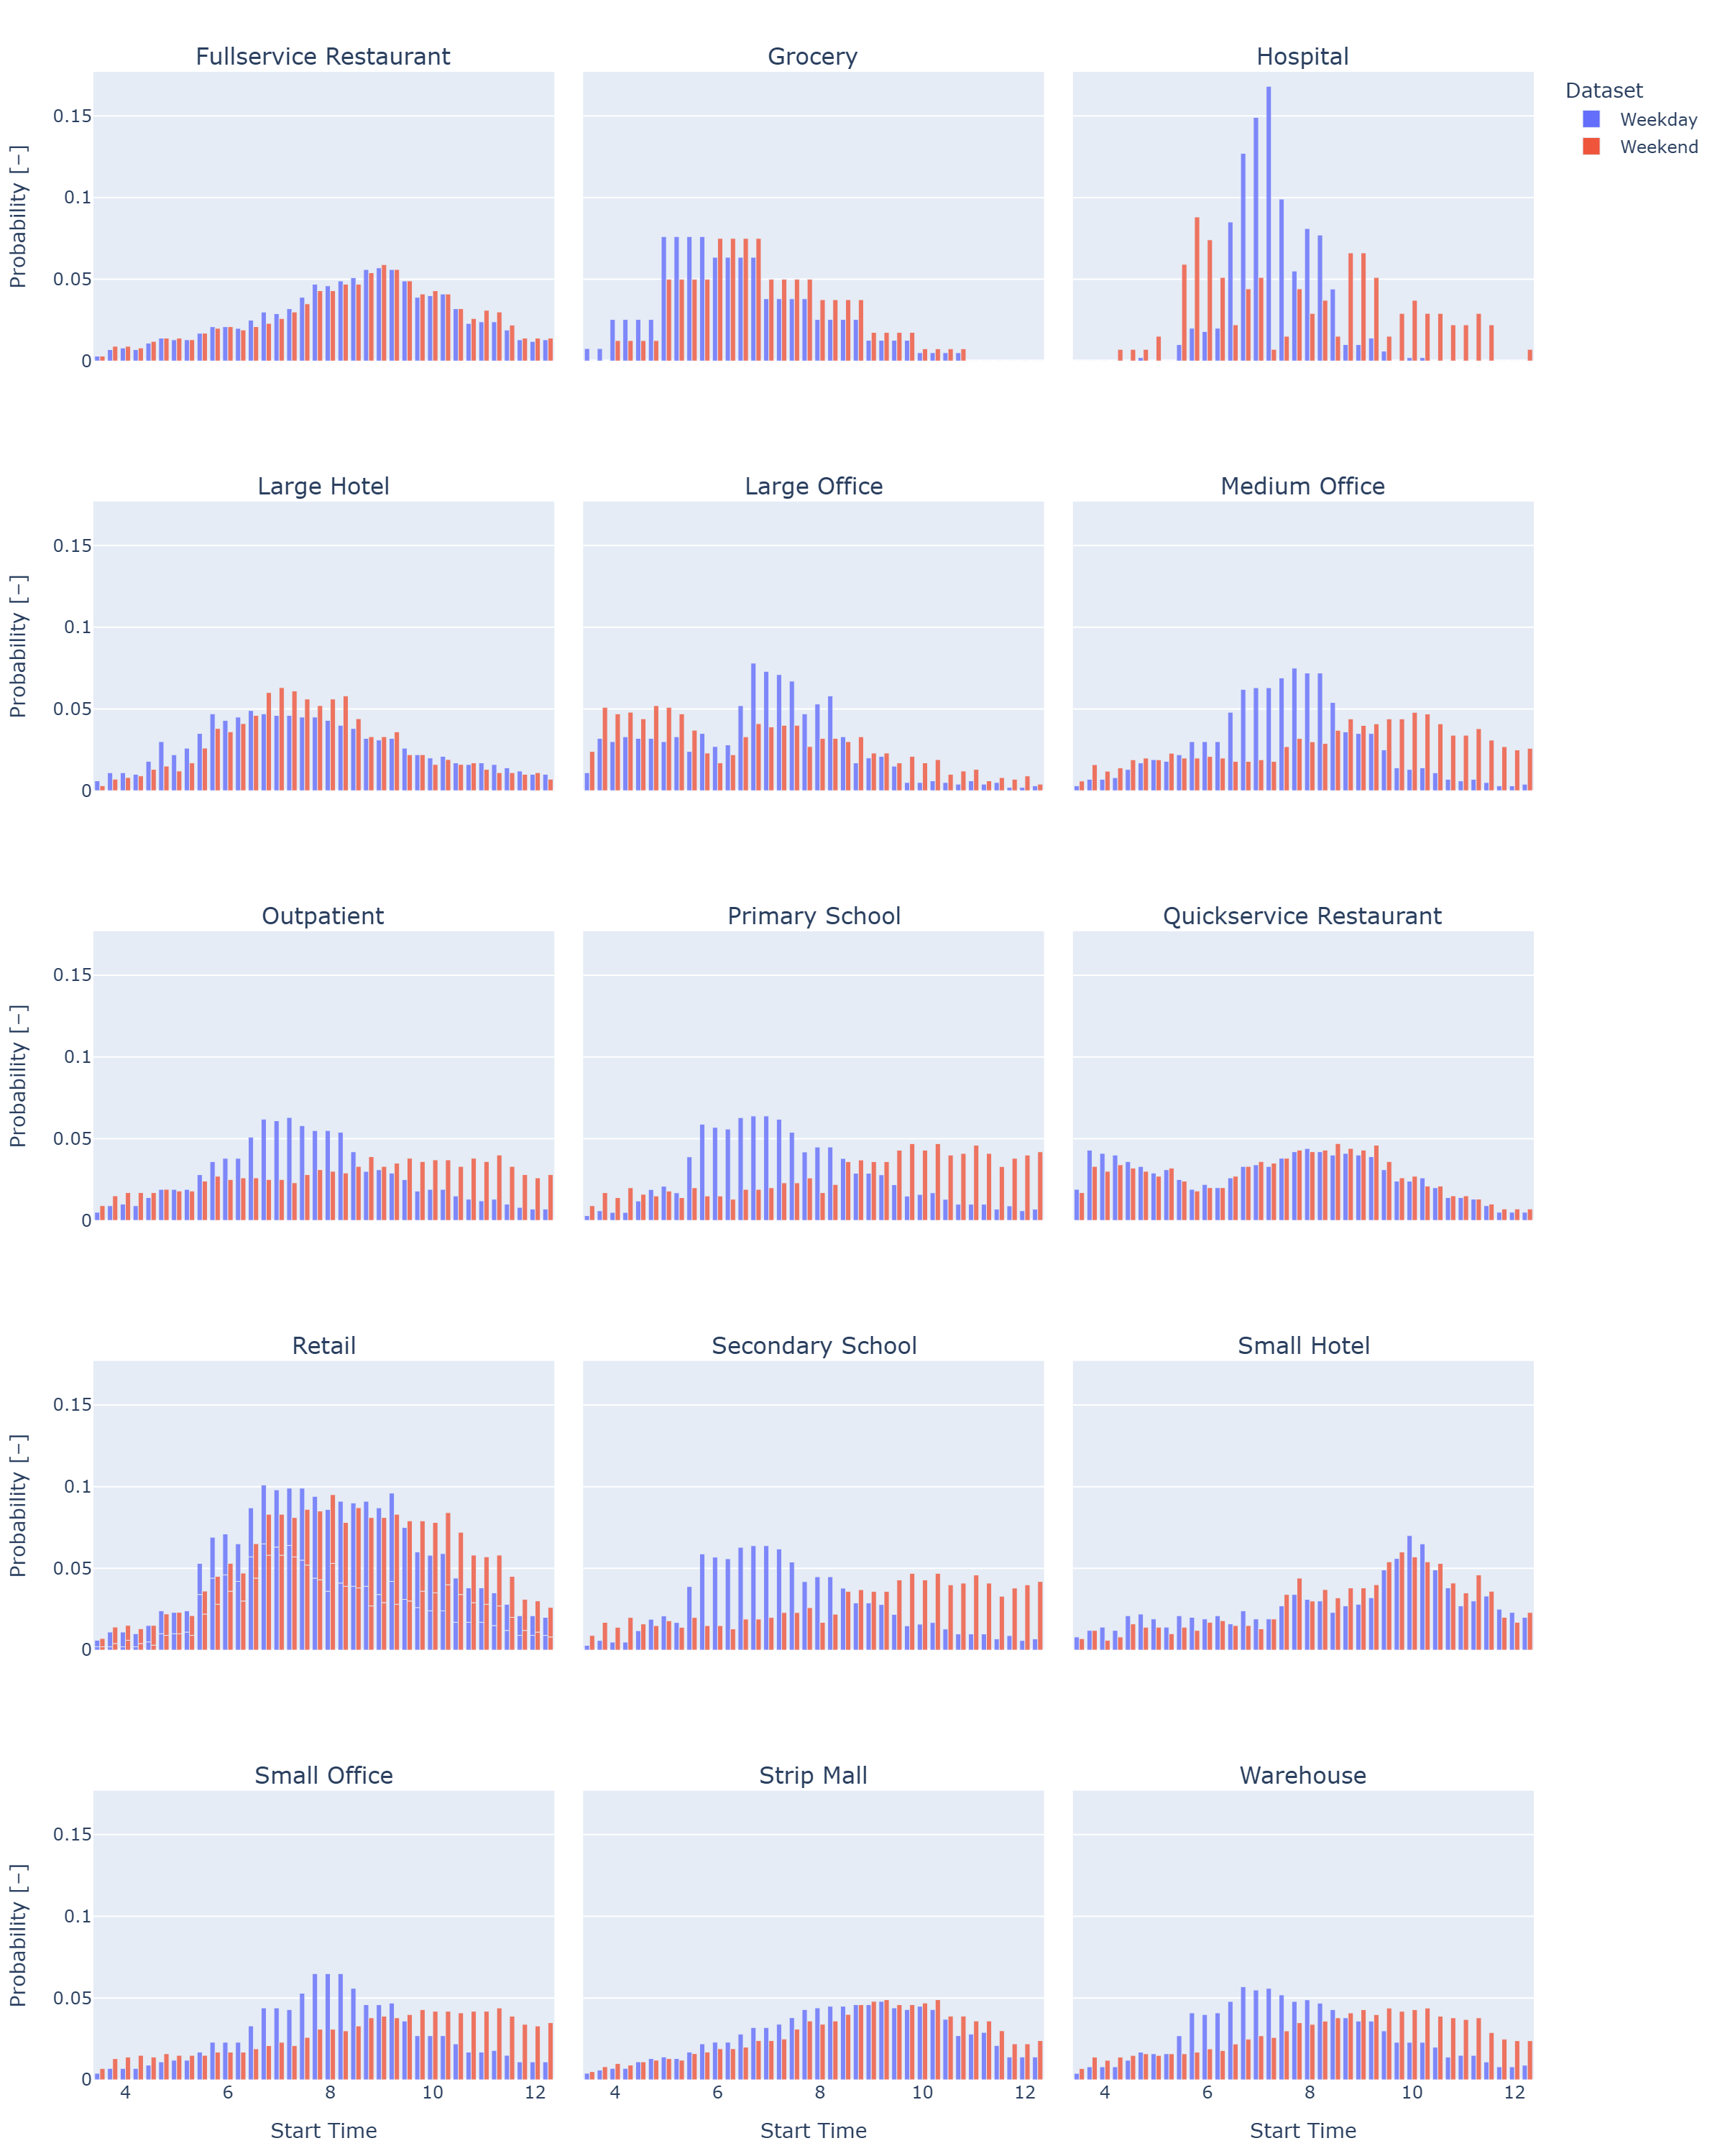
\includegraphics[width=1\textwidth]{figures/start_time.png}
   \caption{Operating hours' start time distributions.}
    \label{fig:start_time}
\end{figure}

\begin{figure}
    \centering 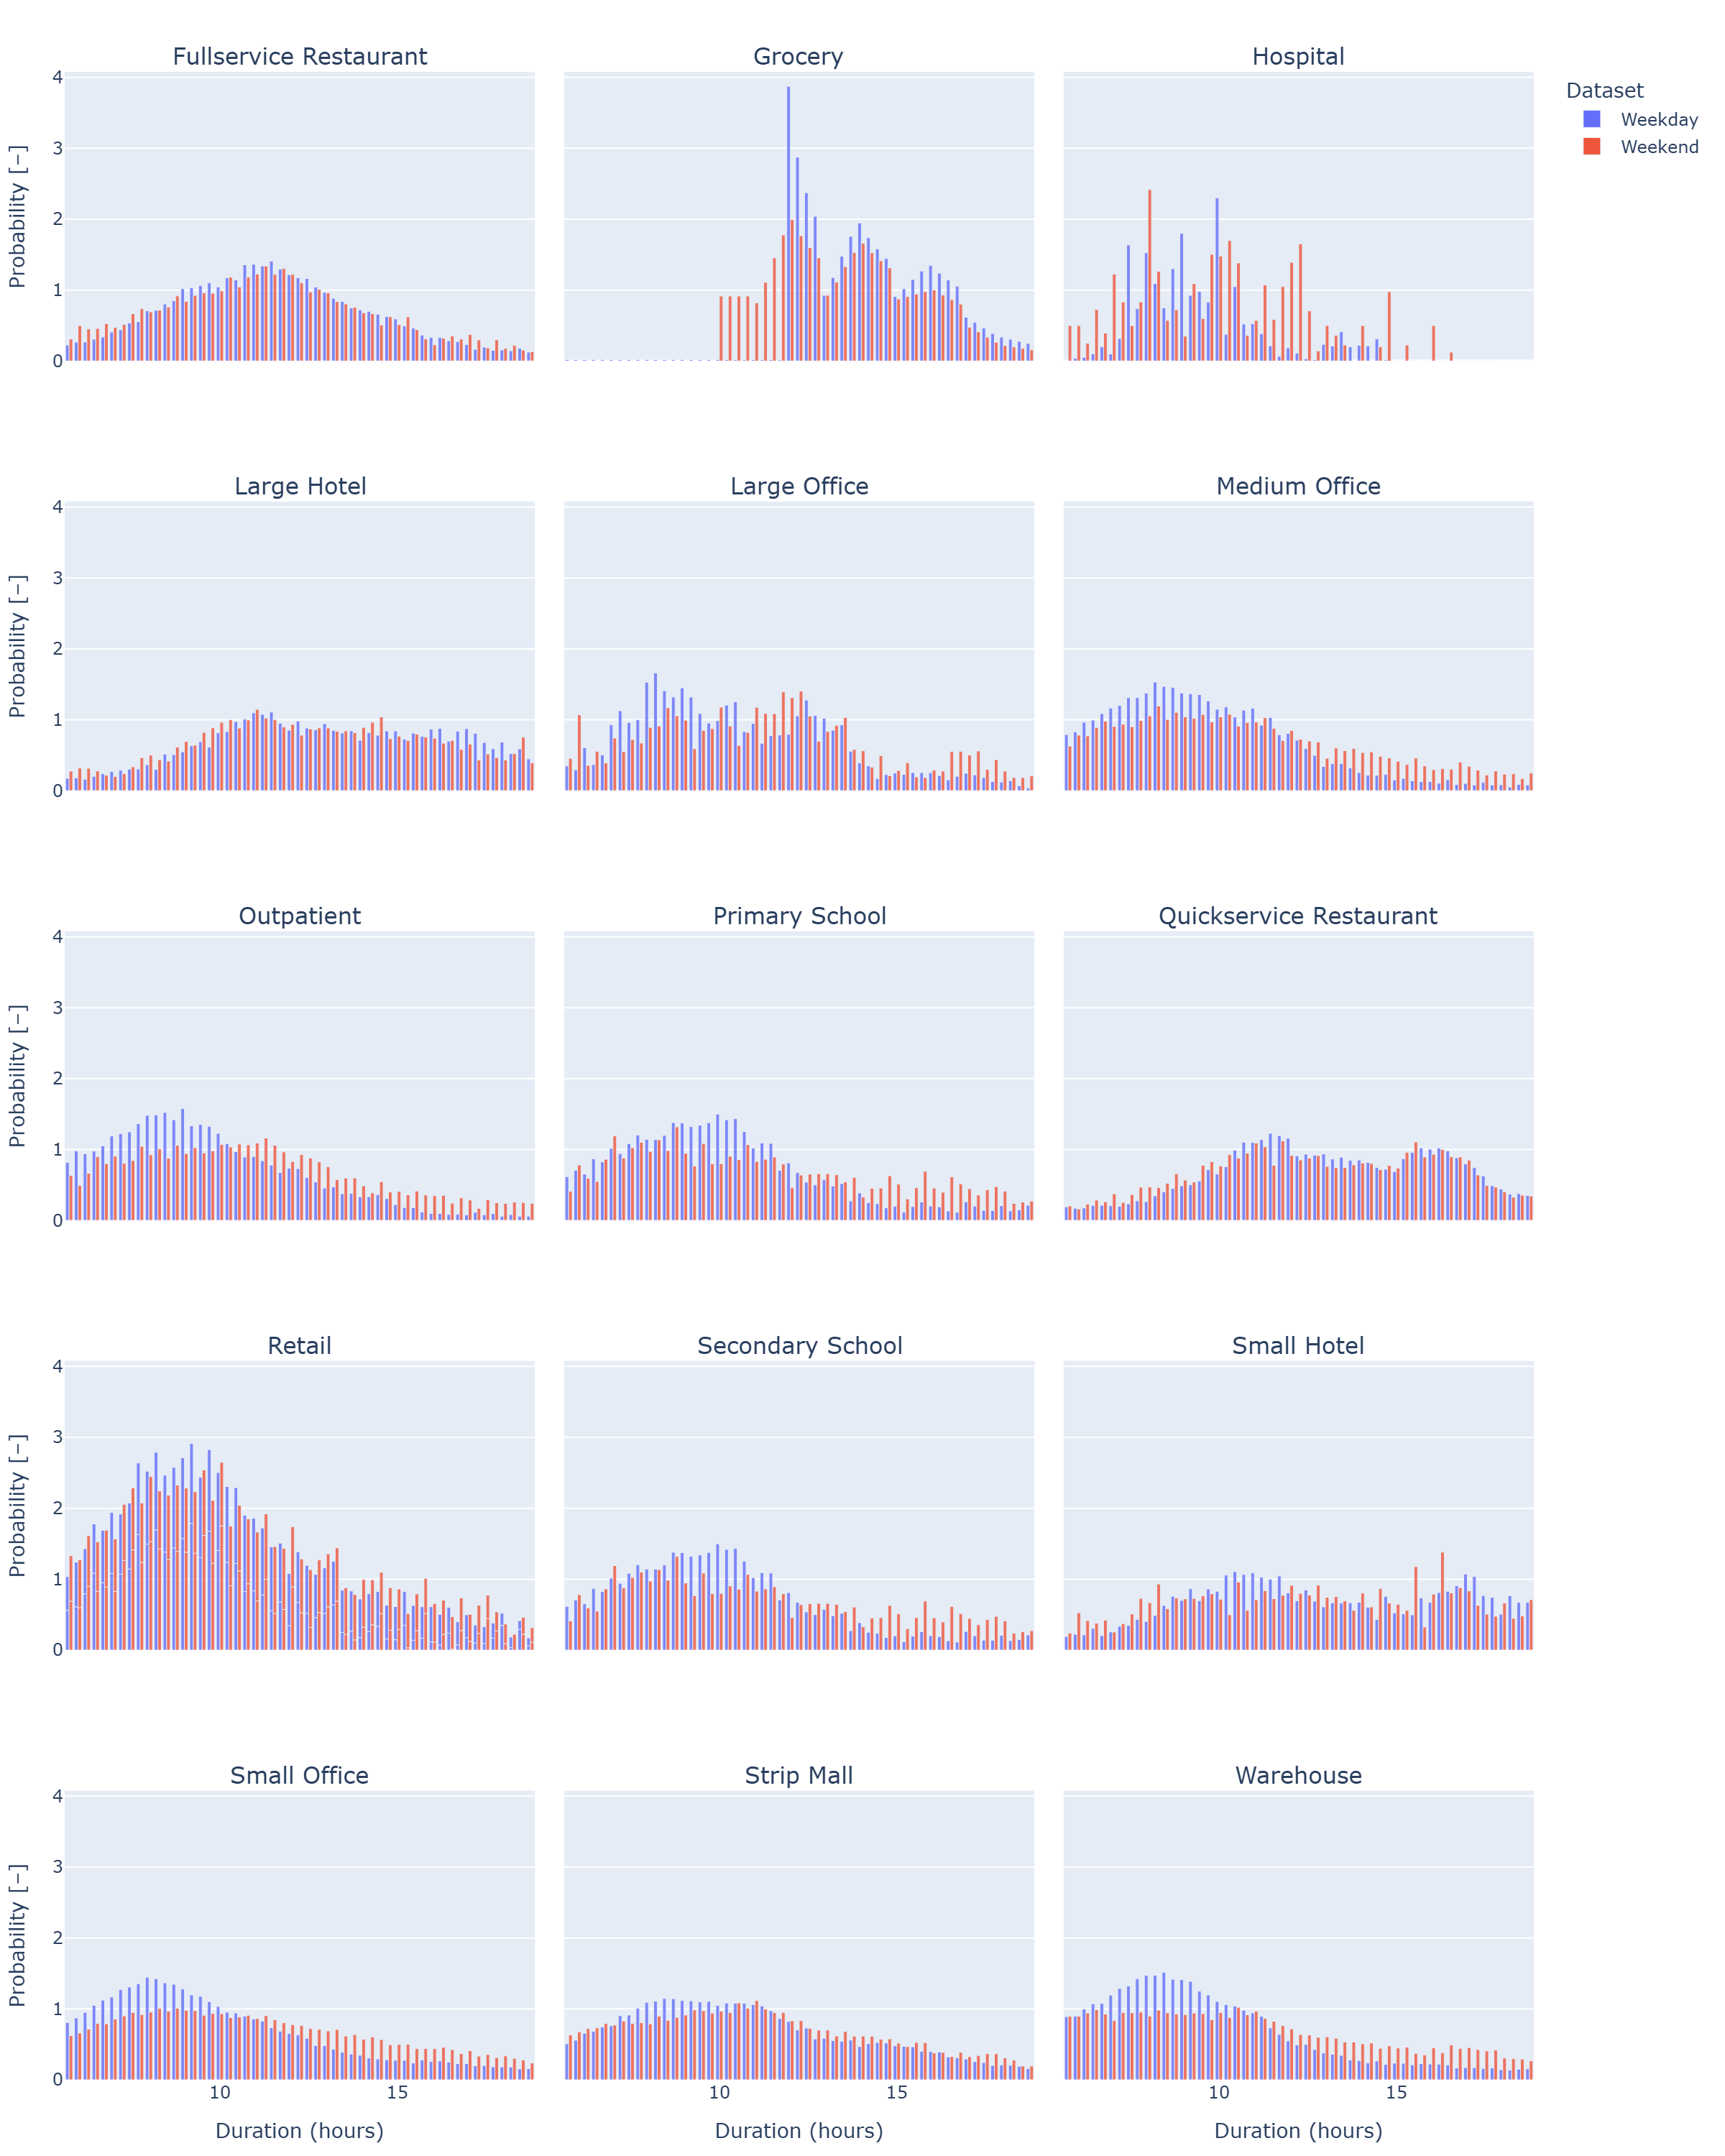
\includegraphics[width=1\textwidth]{figures/duration.png}
    \caption{Operating hours' duration distributions.}
    \label{fig:duration}
\end{figure}

\begin{figure}
    \centering 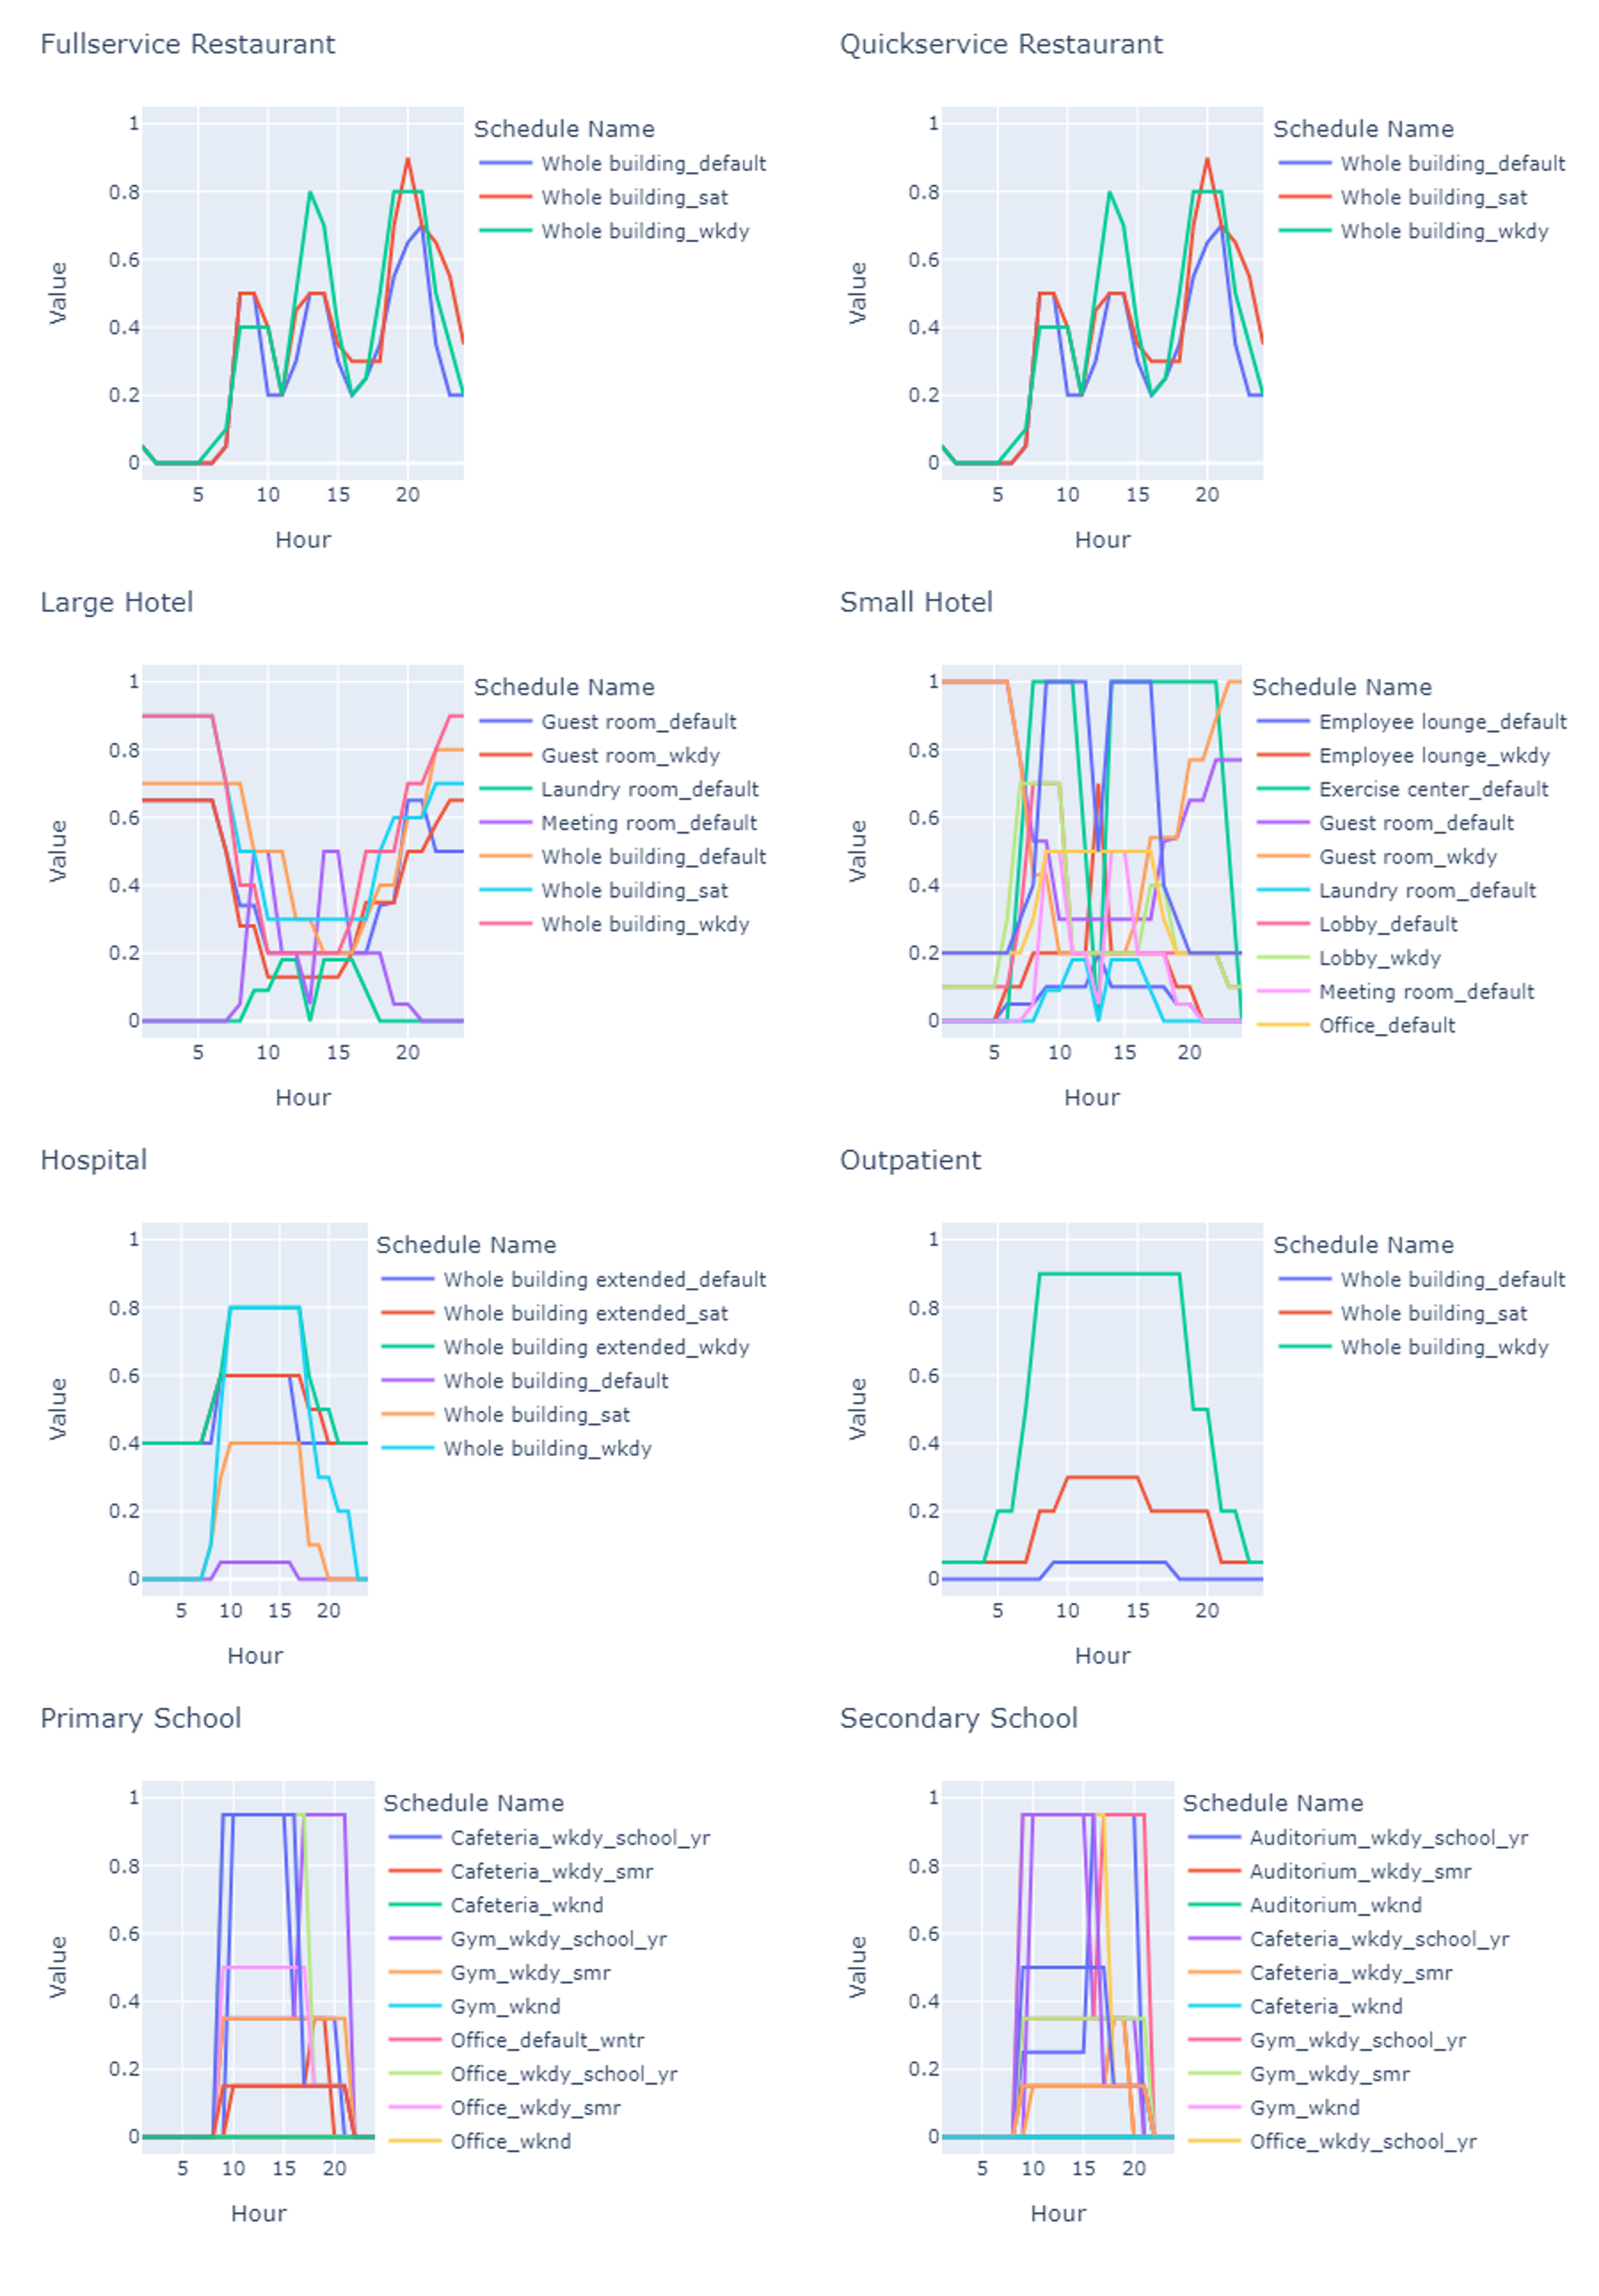
\includegraphics[trim={0 0 0 0}, clip,  % L B R T
    width=0.9\textwidth]{figures/occupancy_schedules_1.png}
    \caption[National base occupancy schedules excluding California]{National base occupancy schedules for food service, lodging, healthcare, and education ComStock building types, excluding California. See Figure \ref{fig:occupancy_schedules_deer_1} for California.}
    \label{fig:occupancy_schedules_1}
\end{figure} 

\begin{figure}
    \centering 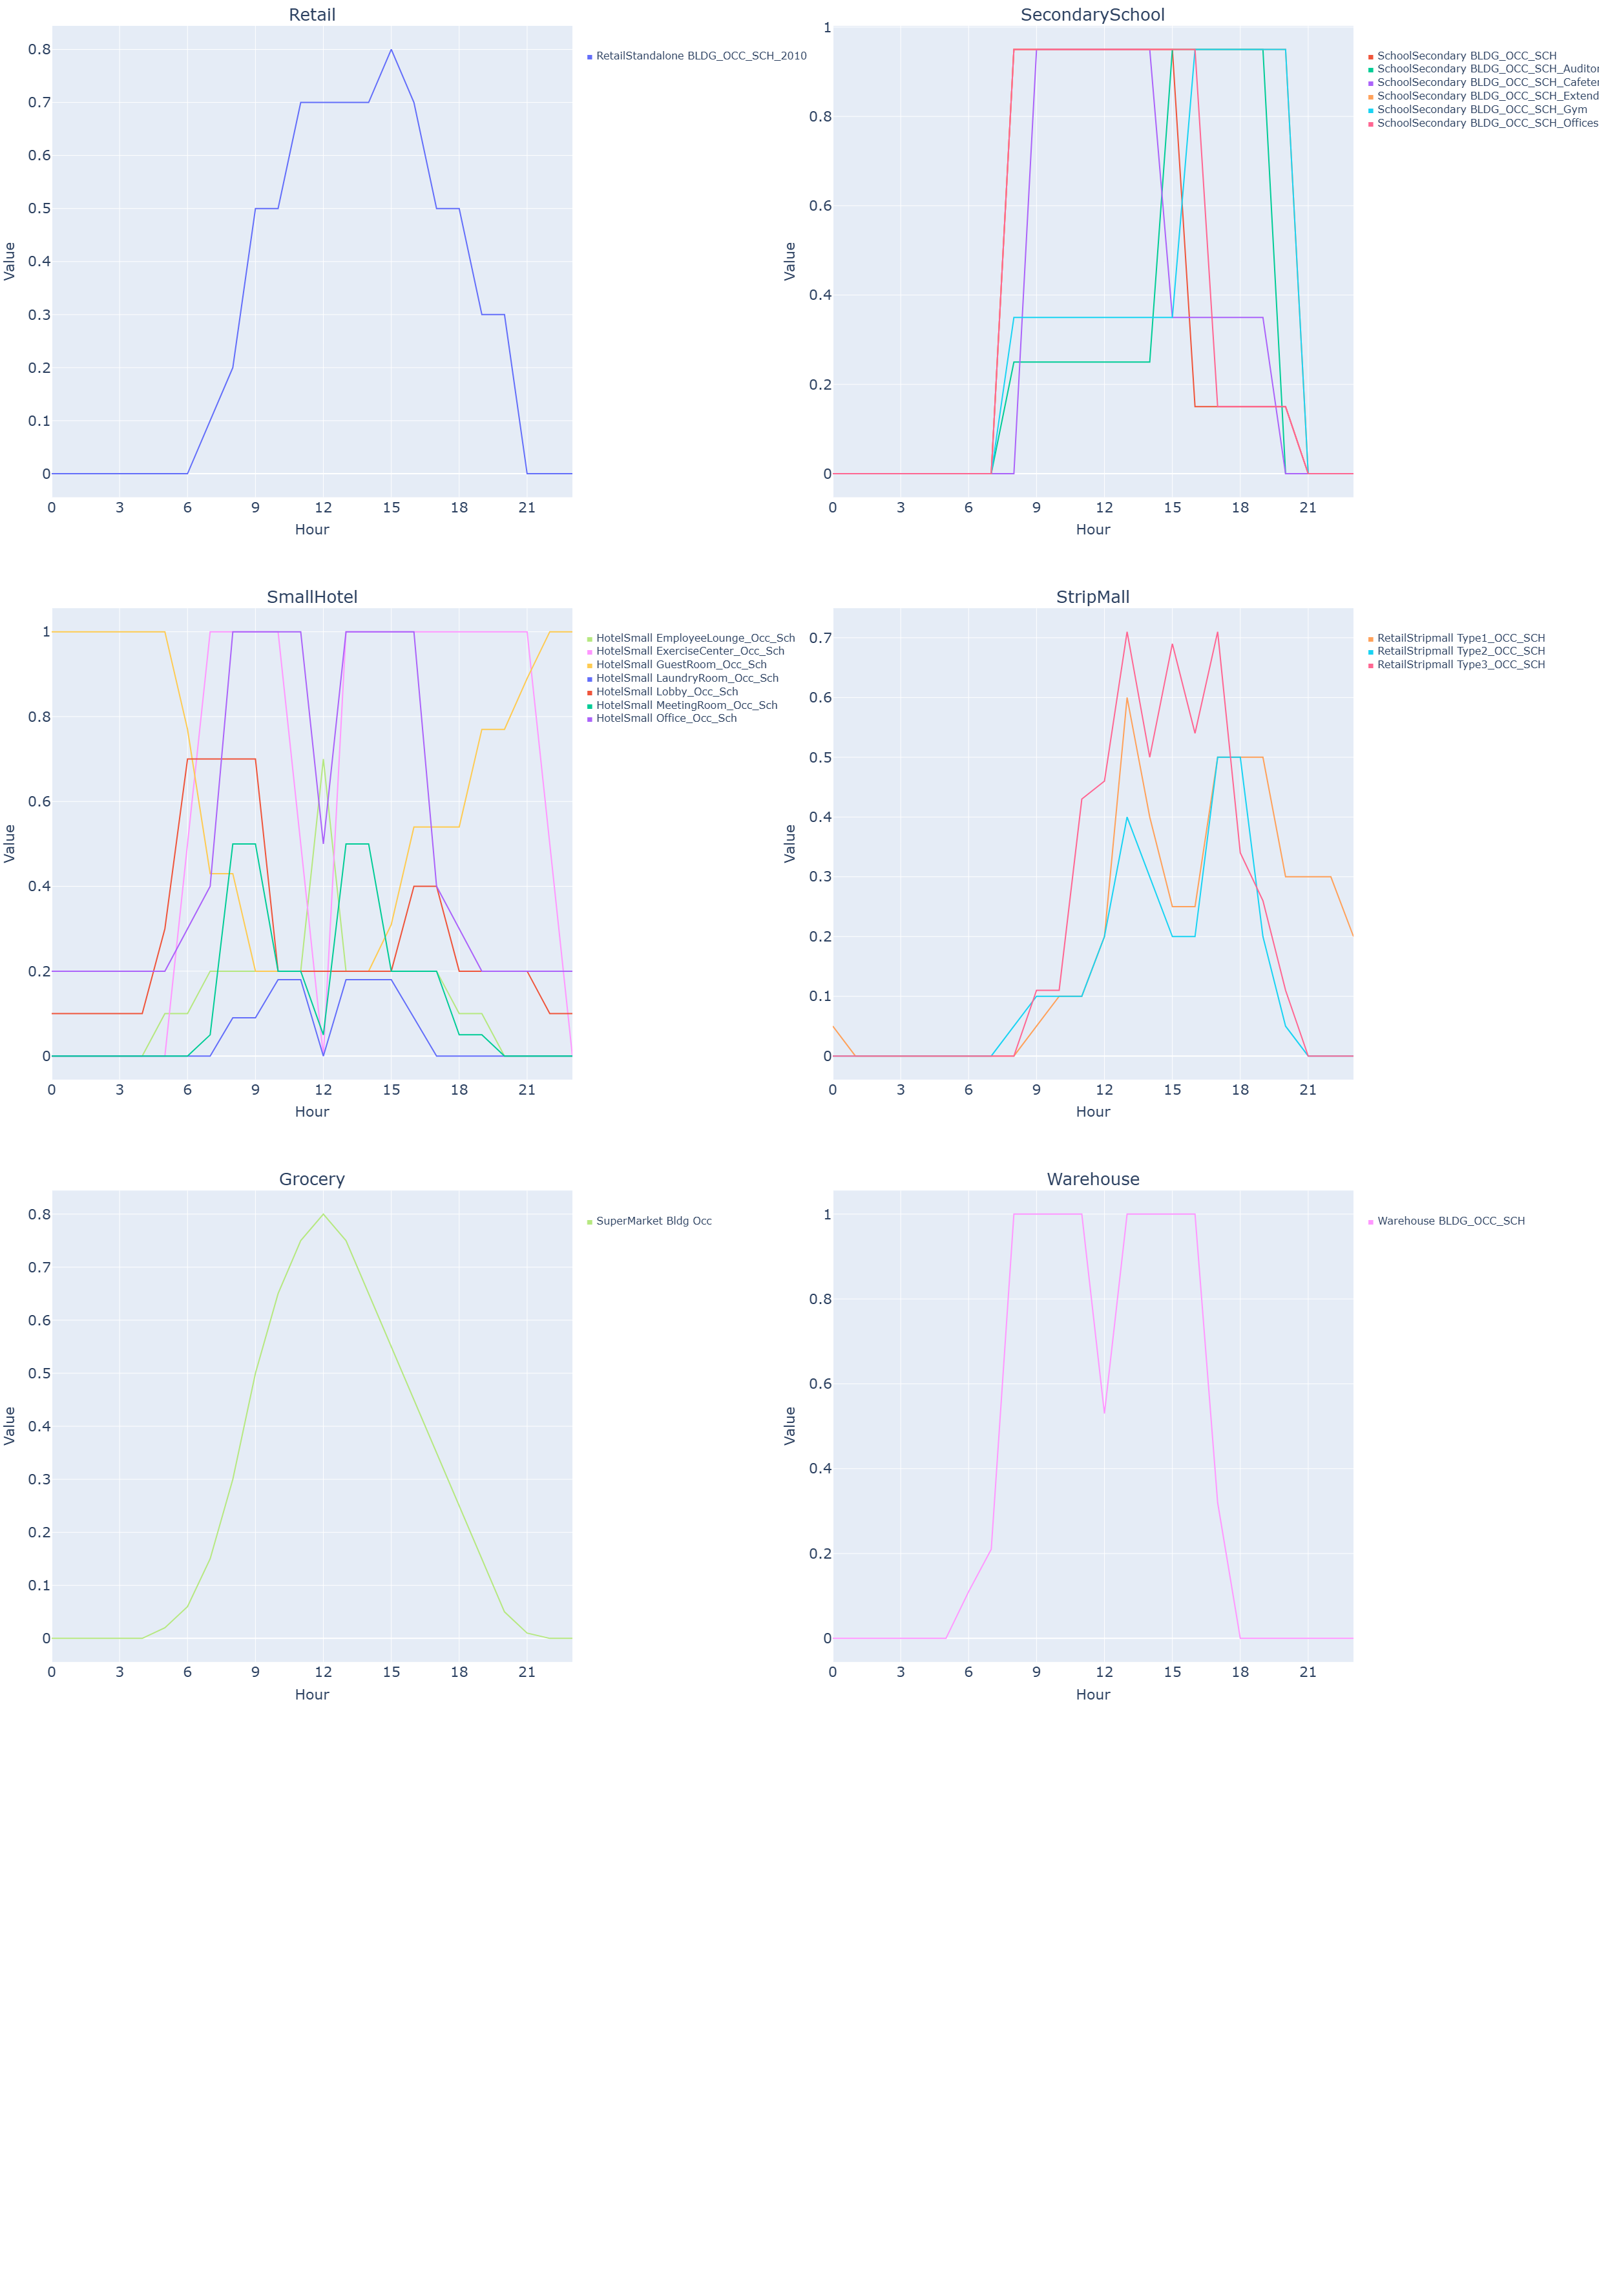
\includegraphics[trim={0 0 0 0}, clip,  % L B R T
    width=0.9\textwidth]{figures/occupancy_schedules_2.png}
    \caption[National base occupancy schedules excluding California]{National base occupancy schedules for retail, office, and warehouse ComStock building types, excluding California. See Figure \ref{fig:occupancy_schedules_deer_2} for California.}
    \label{fig:occupancy_schedules_2}
\end{figure} 